
\documentclass[a4paper,12pt]{report}
\usepackage{a4wide}

%\documentclass[a5paper,10pt]{book}
%\usepackage[top=23mm, bottom=18mm, left=15mm, right=25mm]{geometry}
%\geometry{papersize={170mm,220mm}}


\usepackage[utf8x]{inputenc}
\usepackage[danish]{babel}

\usepackage{xr-hyper} %Externe hyper-ref
\usepackage[colorlinks=true, hyperindex=true, linkcolor=minmblaa, citecolor=minmblaa, urlcolor=minmblaa]{hyperref}
\hypersetup{colorlinks=true,filecolor=minmblaa,bookmarksnumbered=true} %Til hyperreferencer. Referencer med farver
\usepackage{needspace} % giver mulighed for at kræve at der skal være et antal tomme linier på siden før ellers indsættes et sideskift.
\usepackage{framed} %Bokse
\usepackage{wrapfig}

\usepackage{amsmath,amsfonts,amssymb,amsthm,mathtools} %Matematikpakker

\setlength{\parindent}{0mm} %Ingen Indhak i første linje i afsnit

\usepackage{color} %Farvepakke

\usepackage{array}
\usepackage{colortbl}
\usepackage{multirow} %Til at flette rækker i tabeller.

\usepackage{verbatim,mhchem}



	% DOWNLOAD FRA: http://sarovar.org/frs/?group_id=52&release_id=97
	% Læg i directory for hoved TEX fil
%\usepackage[draft]{pdfdraftcopy}
%\draftstring{Licens: Kasper Langt Mellemnavn Skårhøj}
%\draftfontsize{30}
	%\draftfontfamily{hlh}
	%\draftangle{45}
	%\definecolor{mycolor}{rgb}{.825,.855,1}
	%\draftcolor{mycolor}
	%\draftfontattrib



% = Sidehoved =
\usepackage{fancyhdr}
\pagestyle{fancy}
\renewcommand{\sectionmark}[1]{\markright{\protect\titlegraphic{dturoed}\textcolor{dtugraa}{\thesection~\MakeUppercase{#1}}}} % \thesection.\
\fancyhead{}
\fancyfoot{}
\fancyhead[R]{\titlefont\thepage}
\fancyhead[C]{}
\fancyhead[L]{\titlefont \small eNote \MakeUppercase{~\thechapter}~\hspace*{1ex}\rightmark}
\renewcommand\headrulewidth{0pt}
\fancypagestyle{plain}{\fancyfoot[C]{}}% {\titlefont\footnotesize\thepage}}
\setlength{\headheight}{15pt}


% = Længder
%\newlength{\envtblsep}\setlength{\envtblsep}{1\FrameSep}
\newlength{\obsl}\setlength{\obsl}{\textwidth-1.2cm-13.2pt}

% Includes:

% =     Fonts (select one)    =
\usepackage{mathpazo}\linespread{1.05} % Palatino needs more leading (space between lines)
\usepackage{bm} % bold math, must be loaded after the fontpackages

% % Til overskrifter
\DeclareTextFontCommand{\th}{\fontencoding{T1}\fontfamily{phv}\fontseries{b}\selectfont}
\newcommand\titlefont{\fontencoding{T1}\fontfamily{phv}\selectfont}


% =     PGF grafik      =
\usepackage{tikz}
\newcommand\titlegraphic[1]{%
\tikz[baseline] %
\draw[thick,color=#1]
(0pt  ,-0.25em) -- (0pt  ,0.85em)
(2.5pt,-0.25em) -- (2.5pt,0.85em)
(5pt  ,-0.25em) -- (5pt  ,0.85em)
(7.5pt,-0.25em) -- (7.5pt,0.85em);\hspace*{0.8ex} %
}

\newcommand\titlegraphicwide[1]{%
\tikz[baseline] %
\draw[line width=0.8mm,color=#1]
(0pt  ,-0.25em) -- (0pt  ,0.85em)
(4.5pt,-0.25em) -- (4.5pt,0.85em)
(9pt  ,-0.25em) -- (9pt  ,0.85em)
(13.5pt,-0.25em) -- (13.5pt,0.85em);\hspace*{0.8ex} %
}


% =      Title Layout      =
\usepackage{titlesec}
\makeatletter
\titleformat{\chapter}
	[display] % Shape
	{\titlefont\Huge\flushleft} % Title and label format
	{\titlefont\LARGE\bfseries \titlegraphicwide{dturoed}\textcolor{dtugraa}{\@chapapp~\thechapter}} % label
	{0.9em} % label/title separation
	{} % before code
	[] % after code
\makeatother
\titleformat{\section}
	[hang] % Shape
	{\titlefont\Large\flushleft} % Title and label format
	{\thesection} % label
	{0.9em} % label/title separation
	{} % before code
	[] % after code
\titleformat{\subsection}
	[hang] % Shape
	{\titlefont\large} % Title and label format
	{\thesubsection} % label
	{0.9em} % label/title separation
	{} % before code
	[] % after code
\titlespacing{\subsection}{0pt}{*6}{*1.5}
\titleformat{\subsubsection}
	[hang] % Shape
	{\titlefont} % Title and label format
	{\thesubsubsection} % label
	{0.9em} % label/title separation
	{} % before code
	[] % after code



% = Farver
\definecolor{dturoed}{rgb}{0.6, 0.0, 0.0}
\definecolor{dtugraa}{rgb}{0.5, 0.5, 0.5}	% Lidt mørkere. Korrekt = 0.4
\definecolor{mingroenstreg}{rgb}{0.4,0.8,0}	% Sekundærfarve 14 : 102/204/0	(Forårsgrøn) -> Eksempler
\definecolor{mingroen}{rgb}{0.32,0.64,0}		% Sekundærfarve 14, 80% mørkere (tekst)
\definecolor{minorangestreg}{rgb}{1,0.6,0}		% Sekundærfarve 1 : 255/153/0	(Orange) -> Opgaver
\definecolor{minorange}{rgb}{0.8,0.48,0}		% Sekundærfarve 1 , 80% mørkere (tekst)

\definecolor{minblaa}{rgb}{0.2,0.4,0.8}	% Sekundærfarve 13 , 51/102/204 	( Blå -> Definitioner etc)
\definecolor{minmblaa}{rgb}{0.16,0.32,0.64}	% Sekundærfarve 13 , 80% mørkere (tekst)
\definecolor{thmbackground}{rgb}{0.97,.97, 0.99}	% Farve 13 - lys baggrund

\definecolor{mingraastreg}{rgb}{.5,.5,.5}
\definecolor{hvadbackground}{rgb}{0.97,.97, 0.97}
\definecolor{sumgul}{rgb}{1,1,.8}

\definecolor{hjmopgfarve}{rgb}{.96,1,.96}


% = Counter
\newcounter{evncount}[chapter]
\setcounter{evncount}{0}
\renewcommand{\theevncount}{\thechapter.\arabic{evncount}}
\renewcommand{\theequation}{\thechapter-\arabic{equation}}


% = Eksempler = example =
\newenvironment{example}[1][]{
	\refstepcounter{evncount}
	\setlength{\obsl}{\textwidth-1.2cm-13.2pt-9pt} % fix width of the info envirnment%
	\def\FrameCommand{ 
		\textcolor{mingroenstreg}{\vrule width 4pt} 
		\hspace{5pt} 
	}%
	\MakeFramed{\advance\hsize-\width \FrameRestore}%
	\needspace{3\baselineskip}
	\titlegraphic{mingroen}
	\textcolor{mingroen}{
		\th{Eksempel \theevncount \hspace*{5mm} #1}
	} 
	\vspace*{3mm}%
	\begin{small}
	\par
}
{
	\end{small}
	\endMakeFramed
}


% = Opgaver = exercise =
\newenvironment{exercise}[1][]{
	\refstepcounter{evncount}
	\setlength{\obsl}{\textwidth-1.2cm-13.2pt-9pt}% fix width of the info envirnment%
	\def\FrameCommand{
		\textcolor{minorangestreg}{\vrule width 4pt}
		\hspace{5pt}
	}%
	\MakeFramed{\advance\hsize-\width \FrameRestore}%
	\needspace{3\baselineskip}
	\titlegraphic{minorange}
	\textcolor{minorange}{
		\th{Opgave \theevncount \hspace*{5mm} #1}
	} 
	\vspace*{3mm}%
	\begin{small}
	\par
}
{
	\end{small}
	\endMakeFramed
}


% = Bevis
\newenvironment{bevis}{
	\setlength{\obsl}{\textwidth-1.2cm-13.2pt-9pt} % fix width of the info envirnment%
	\def\FrameCommand{
		\textcolor{mingraastreg}{\vrule width 4pt} 
		\hspace{5pt}
	}%
	\MakeFramed{\advance\hsize-\width \FrameRestore}%
	\needspace{3\baselineskip}
	\titlegraphic{black}
	\textcolor{black}{
		\th{Bevis}
	}
	\vspace*{3mm}%
	\begin{small}
	\par
}
{
	\bevisslut 
	\end{small}
	\endMakeFramed
}


% = Definition =
\newenvironment{definition}[1][]{
	\vspace{4mm}
	\pagebreak[1]
	\setlength{\obsl}{\textwidth-1.2cm-2\FrameSep-13.2pt}%
	\def\FrameCommand{
		\fboxsep=\FrameSep\fcolorbox{minblaa}{thmbackground}
	}
	\begin{minipage}{\textwidth}
	\MakeFramed{\advance\hsize-\width\FrameRestore}
	\refstepcounter{evncount}
	\titlegraphic{minblaa}
	\textcolor{minmblaa}{
		\th{Definition \theevncount \hspace*{5mm} #1}
	}
	\vspace*{3mm}
	\par
}
{
	\endMakeFramed 
	\end{minipage}
	\vspace{4mm}
}


% = Theorem =
\newenvironment{theorem}[1][]{
	\vspace{4mm}
	\pagebreak[1]%
	\setlength{\obsl}{\textwidth-1.2cm-2\FrameSep-13.2pt}%
	\def\FrameCommand{
		\fboxsep=\FrameSep\fcolorbox{minblaa}{thmbackground}
	}%
	\begin{minipage}{\textwidth}
	\MakeFramed{\advance\hsize-\width\FrameRestore}%
	\refstepcounter{evncount}
	\titlegraphic{minblaa}
	\textcolor{minmblaa}{
		\th{Sætning \theevncount \hspace*{5mm} #1}
	}
	\vspace*{3mm}
	\par
}
{
	\endMakeFramed 
	\end{minipage}
	\vspace{4mm}
}


% = Lemma =
\newenvironment{lemma}[1][]{
	\vspace{4mm}
	\pagebreak[1]
	\setlength{\obsl}{\textwidth-1.2cm-2\FrameSep-13.2pt}%
	\def\FrameCommand{
		\fboxsep=\FrameSep \fcolorbox{minblaa}{thmbackground}
	}
	\begin{minipage}{\textwidth} 
	\MakeFramed{\advance\hsize-\width \FrameRestore}
	\refstepcounter{evncount}
	\titlegraphic{minblaa}
	\textcolor{minmblaa}{
		\th{Hjælpesætning \theevncount \hspace*{5mm} #1}
	}
	\vspace*{3mm}
	\par
}
{
	\endMakeFramed 
	\end{minipage}
	\vspace{4mm}
}


% = Corollary =
\newenvironment{corollary}[1][]{
	\vspace{4mm}
	\pagebreak[1]
	\setlength{\obsl}{\textwidth-1.2cm-2\FrameSep-13.2pt}%
	\def\FrameCommand{
		\fboxsep=\FrameSep \fcolorbox{minblaa}{thmbackground}
	}
	\begin{minipage}{\textwidth} 
	\MakeFramed{\advance\hsize-\width \FrameRestore}
	\refstepcounter{evncount}
	\titlegraphic{minblaa}
	\textcolor{minmblaa}{
		\th{Følgesætning \theevncount \hspace*{5mm} #1}
	}
	\vspace*{3mm}
	\par
}
{
	\endMakeFramed 
	\end{minipage}
	\vspace{4mm}
}


% = Metode = method
\newenvironment{method}[1][]{
	\vspace{4mm}
	\pagebreak[1]
	\setlength{\obsl}{\textwidth-1.2cm-2\FrameSep-13.2pt}%
	\def\FrameCommand{
		\fboxsep=\FrameSep \fcolorbox{black}{hvadbackground}
	}
	\begin{minipage}{\textwidth} 
	\MakeFramed{\advance\hsize-\width \FrameRestore}
	\refstepcounter{evncount}
	\titlegraphic{black}
	\textcolor{black}{
		\th{Metode \theevncount \hspace*{5mm} #1}
	}
	\vspace*{3mm}
	\par
}
{
	\endMakeFramed
	\end{minipage}
	\vspace{4mm}
}


% = Forklaring = explain =
\newenvironment{explain}[1][]{
	\vspace{4mm}
	\pagebreak[1]
	\setlength{\obsl}{\textwidth-1.2cm-2\FrameSep-13.2pt}%
	\def\FrameCommand{
		\fboxsep=\FrameSep \fcolorbox{black}{hvadbackground}
	}
	\MakeFramed{\advance\hsize-\width \FrameRestore}
	\refstepcounter{evncount}
	\titlegraphic{black}
	\textcolor{black}{
		\th{Forklaring \theevncount \hspace*{5mm} #1}
	}
	\vspace*{3mm}
	\par
}
{
	\endMakeFramed
	\vspace{4mm}
}


% = Bemærkning = remark =
\newenvironment{remark}[1][]{
	\vspace{4mm}
	\pagebreak[1]
	\setlength{\obsl}{\textwidth-1.2cm-2\FrameSep-13.2pt}%
	\def\FrameCommand{
		\fboxsep=\FrameSep \fcolorbox{black}{hvadbackground}
	}
	\begin{minipage}{\textwidth} 
	\MakeFramed{\advance\hsize-\width \FrameRestore}
	\refstepcounter{evncount}
	\titlegraphic{black}
	\textcolor{black}{
		\th{Bemærkning \theevncount \hspace*{5mm} #1}
	}
	\vspace*{3mm}
	\par
}
{
	\endMakeFramed 
	\end{minipage}
	\vspace{4mm}
}







% = OBS! = obs =
\newenvironment{obs}{\vspace{4mm}\par%
\begin{tabular}{m{1.2cm}<{\hspace*{2mm}}@{}|m{\obsl}@{}}\hspace*{-4pt}\raggedleft
\includegraphics[width=1.1cm]{../Strukturfiler/FIGS/Alert01} & \begin{minipage}{\obsl}}{\end{minipage}\\ \end{tabular}\vspace{4mm}\par}


% = INFO = info =
\newenvironment{info}{\vspace{4mm}\par%
\begin{tabular}{m{1.2cm}<{\hspace*{2mm}}@{}|m{\obsl}@{}}\hspace*{-4pt}\raggedleft
\includegraphics[width=1.1cm]{../Strukturfiler/FIGS/Info01} & \begin{minipage}{\obsl}}{\end{minipage}\\ \end{tabular}\vspace{4mm}\par}


% = THINK= think =
\newenvironment{think}{\vspace{4mm}\par%
\begin{tabular}{m{1.2cm}<{\hspace*{2mm}}@{}|m{\obsl}@{}}\hspace*{-4pt}\raggedleft
\includegraphics[width=0.7cm]{../Strukturfiler/FIGS/ChessPiece} & \begin{minipage}{\obsl}}{\end{minipage}\\ \end{tabular}\vspace{4mm}\par}


% = AHA= aha =
\newenvironment{aha}{\vspace{4mm}\par%
\begin{tabular}{m{1.2cm}<{\hspace*{2mm}}@{}|m{\obsl}@{}}\hspace*{-4pt}\raggedleft
\includegraphics[width=1.1cm]{../Strukturfiler/FIGS/Think} & \begin{minipage}{\obsl}}{\end{minipage}\\ \end{tabular}\vspace{4mm}\par}


% = BUILDUP= build =
\newenvironment{build}{\vspace{4mm}\par%
\begin{tabular}{m{1.2cm}<{\hspace*{2mm}}@{}|m{\obsl}@{}}\hspace*{-4pt}\raggedleft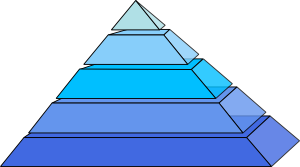
\includegraphics[width=1.1cm]{../Strukturfiler/FIGS/BluePyramid} & \begin{minipage}{\obsl}}{\end{minipage}\\ \end{tabular}\vspace{4mm}\newline}


% = Forudsætning = basis
\newenvironment{basis}{\begin{flushleft} \begin{itshape} }{\end{itshape} \end{flushleft}}


% = Opsummering =
\newenvironment{summary}{\clearpage\pagecolor{sumgul}\section{Opsummering}}{\newpage\pagecolor{white}}











% = Counter
\newcounter{opgavecount}[section]
\setcounter{opgavecount}{0}
\newcounter{spgcount}[opgavecount]
\setcounter{spgcount}{0}
\renewcommand{\thespgcount}{\alph{spgcount})}



% = EXERCISE = (DIVIDER)

\newcommand{\exercisebegin}[1][]{\bigskip\needspace{3\baselineskip}\refstepcounter{opgavecount}\titlegraphic{mingroen}\textcolor{mingroen}{\th{Opgave \theopgavecount \hspace*{1cm} #1}}\medskip\par}

% = QUIZEXERCISE = (DIVIDER)

\newcommand{\quizexercisebegin}[1][]{\bigskip\needspace{3\baselineskip}\refstepcounter{opgavecount}\titlegraphic{mingroen}\textcolor{mingroen}{\th{Quiz-Opgave \theopgavecount \hspace*{1cm} #1}}\medskip\par}

% = QUESTION =

\newenvironment{question}{\refstepcounter{spgcount}\begin{itemize}\item[\thespgcount]}{\end{itemize}\hspace*{\fill}}

% = VINK =

\newenvironment{vink}{\begin{tabular}{m{.9cm}<{\hspace*{2mm}}@{}|m{\obsl}@{}}\hspace*{-4pt}\raggedleft
\includegraphics[width=.9cm]{../Strukturfiler/FIGS/Think} & \begin{minipage}{\obsl}}{\end{minipage}\\ \end{tabular}\medskip\\}
	
% = FACIT =

\newenvironment{facit}{\begin{tabular}{m{.9cm}<{\hspace*{2mm}}@{}|m{\obsl}@{}}\hspace*{-4pt}\raggedleft
\includegraphics[width=.9cm]{../Strukturfiler/FIGS/Check} & \begin{minipage}{\obsl}}{\end{minipage}\\ \end{tabular}\medskip\\}








\newcommand{\afsnit}[1]{\bigskip\th{\titlegraphic{mingroen}\textcolor{mingroen}{#1}} \\ \rule[7pt]{.4\textwidth}{1pt} \vspace*{-2.5mm}\par}

% (DIVIDER):
\newcommand{\ugedagdatotitel}[4]{\pagebreak[4]\section{Semesteruge #1 -- #2 Dag \hspace*{1mm} (#3)} \vspace*{-4mm} \rule[5pt]{\textwidth}{1pt}\vspace*{-2.5mm} \begin{center}\large{\th{#4}}\end{center} \fancyhead[C]{\th{Semesteruge #1}}}

\newenvironment{skema}[1]{\definecolor{shadecolor}{rgb}{0.96,.98, 1.0} \setlength{\FrameSep}{6pt} \renewcommand{\FrameHeightAdjust}{10pt} \vspace*{-4pt}\begin{shaded} \begin{tabular}{#1}}{\end{tabular} \end{shaded} \vspace*{-7pt}}


% ========================

% MAKROER

%\newenvironment{matr}[1][]{\hspace*{-.8mm}\left[\hspace*{-1mm}\begin{array}{#1}}{\end{array}\hspace*{-1mm}\right]\hspace*{-.8mm}}
\newcommand{\bevisslut}{\begin{scriptsize} \begin{flushright} $ \blacksquare $ \end{flushright} \end{scriptsize}}

\newcommand{\tref}[2]{\hyperref[#1]{#2 \ref*{#1}}}
\newcommand{\thref}[2]{\hyperref[#1]{#2}}

\newcommand{\refA}[1]{\colorbox{yellow}{\ref{#1}}}
\newcommand{\hrefA}[2]{\colorbox{yellow}{\href{#1}{#2}}}
\newcommand{\trefA}[2]{\colorbox{yellow}{\hyperref[#1]{#2 \ref*{#1}}}}
\newcommand{\threfA}[2]{\colorbox{yellow}{\hyperref[#1]{#2}}}

\newenvironment{matr}[1]{\hspace*{-.8mm}\begin{bmatrix}\hspace*{-1mm}\begin{array}{#1}}{\end{array}\hspace*{-1mm}\end{bmatrix}\hspace*{-.8mm}}
\newcommand{\transp}{\hspace*{-.6mm}^{\top}}

\newcommand{\maengde}[2]{\left\lbrace \hspace*{-1mm} \begin{array}{c|c} #1 & #2 \end{array} \hspace*{-1mm} \right\rbrace}

\newenvironment{eqnalign}[1]{\setlength{\arraycolsep}{1.3pt}\begin{equation}\begin{array}{#1}}{\end{array}\end{equation}\par}
\newcommand{\eqnl}{\setlength{\arraycolsep}{1.3pt}}

\newcommand{\matind}[3]{{_\mathrm{#1}\mathbf{#2}_\mathrm{#3}}}
\newcommand{\vekind}[2]{{_\mathrm{#1}\mathbf{#2}}}
\newcommand{\jac}[2]{{\mathrm{Jacobi}_\mathbf{#1} (#2)}}
\newcommand{\diver}[2]{{\mathrm{div}\mathbf{#1} (#2)}}
\newcommand{\rot}[1]{{\mathbf{rot}\mathbf{(#1)}}}

\newcommand{\am}{\mathrm{am}}
\newcommand{\gm}{\mathrm{gm}}
\newcommand{\E}{\mathrm{E}}
\newcommand{\Span}{\mathrm{span}}
\newcommand{\mU}{\mathbf{U}}

\newcommand{\ms}{\medskip\\}
\newcommand{\bs}{\bigskip\\}

\newcommand{\mA}{\mathbf{A}}
\newcommand{\mB}{\mathbf{B}}
\newcommand{\mC}{\mathbf{C}}
\newcommand{\mD}{\mathbf{D}}
\newcommand{\mE}{\mathbf{E}}
\newcommand{\mF}{\mathbf{F}}
\newcommand{\mK}{\mathbf{K}}
\newcommand{\mI}{\mathbf{I}}
\newcommand{\mM}{\mathbf{M}}
\newcommand{\mN}{\mathbf{N}}
\newcommand{\mQ}{\mathbf{Q}}
\newcommand{\mT}{\mathbf{T}}
\newcommand{\mV}{\mathbf{V}}
\newcommand{\mW}{\mathbf{W}}
\newcommand{\mX}{\mathbf{X}}
\newcommand{\ma}{\mathbf{a}}
\newcommand{\mb}{\mathbf{b}}
\newcommand{\mc}{\mathbf{c}}
\newcommand{\md}{\mathbf{d}}
\newcommand{\me}{\mathbf{e}}
\newcommand{\mn}{\mathbf{n}}
\newcommand{\mr}{\mathbf{r}}
\newcommand{\mv}{\mathbf{v}}
\newcommand{\mw}{\mathbf{w}}
\newcommand{\mx}{\mathbf{x}}
\newcommand{\mxb}{\mathbf{x_{bet}}}
\newcommand{\my}{\mathbf{y}}
\newcommand{\mz}{\mathbf{z}}
\newcommand{\reel}{\mathbb{R}}
\newcommand{\mL}{\bm{\Lambda}} %Lambda-matrix
\newcommand{\mnul}{\bm{0}}
\newcommand{\trap}[1]{\mathrm{trap}(#1)}
\newcommand{\Det}{\operatorname{Det}}
\newcommand{\adj}{\operatorname{adj}}
\newcommand{\Ar}{\operatorname{Areal}}
\newcommand{\Vol}{\operatorname{Vol}}
\newcommand{\Rum}{\operatorname{Rum}}
\newcommand{\diag}{\operatorname{\bf{diag}}}
\newcommand{\bidiag}{\operatorname{\bf{bidiag}}}
\newcommand{\spanVec}[1]{\mathrm{span}\{#1\}}
\newcommand{\Div}{\operatorname{Div}}
\newcommand{\Rot}{\operatorname{\mathbf{Rot}}}

\newcommand{\Jac}{\operatorname{Jacobi}}
\newcommand{\Tan}{\operatorname{Tan}}
\newcommand{\Ort}{\operatorname{Ort}}
\newcommand{\Flux}{\operatorname{Flux}}
\newcommand{\Cmass}{\operatorname{Cm}}
\newcommand{\Imom}{\operatorname{Im}}
\newcommand{\Pmom}{\operatorname{Pm}}
\newcommand{\IS}{\operatorname{I}}
\newcommand{\IIS}{\operatorname{II}}
\newcommand{\IIIS}{\operatorname{III}}
\newcommand{\Le}{\operatorname{L}}
\newcommand{\app}{\operatorname{app}}
\newcommand{\M}{\operatorname{M}}
\newcommand{\re}{\mathrm{Re}}
\newcommand{\im}{\mathrm{Im}}

\newcommand{\compl}{\mathbb{C}} %de komplekse tal
\newcommand{\e}{\mathrm{e}} %eksponentialfunktionen. lodret 'e', og altså ikke kursiv ligesom andre bogstaver.





% Medialink: SCREEN: (QRcode) + thumbnail image + link på kodenummer (til qr.dtu.dk)
\newcommand{\onlinemedia}[3]{
	\begin{wrapfigure}{r}{3.2cm} 
		\vspace{-30pt} 
		\vspace{#1pt} 
		\begin{flushright} 
			\includegraphics[width=3cm]{qr/#2.png} 
			\tiny 
			\href{http://qr.dtu.dk/#2}{#2: #3}
			\normalsize  
		\end{flushright} 
		\vspace{-10pt} 
	\end{wrapfigure}
}
\newcommand{\onlinemediathumb}[3]{
	\begin{wrapfigure}{r}{3.2cm} 
		\vspace{-30pt} 
		\vspace{#1pt} 
		\begin{flushright} 
			\includegraphics[width=3cm]{qr/#2.png} 
			\includegraphics[width=3cm]{qr/#2_thumb.png} 
			\tiny 
			\href{http://qr.dtu.dk/#2}{#2: #3}
			\normalsize  
		\end{flushright} 
		\vspace{-10pt} 
	\end{wrapfigure}
}



% Index:
\usepackage{makeidx}
\makeindex
\newcommand\ind[2]{\index{#1}\textbf{\textit{\textcolor{black}{#2}}}}

% ###SERVER_EXCLUDE_BEGIN###
\externaldocument[NUID17-]{../../enoten/TN01-Talrum/Talrum}
\externaldocument[NUID1-]{../../enoten/TN02-Ligningssystemer/TNdriver}
\externaldocument[NUID2-]{../../enoten/TN03-Matricer_og_Matrixalgebra/Matricer_og_matrixalgebra}
\externaldocument[NUID3-]{../../enoten/TN04-Kvadratiske_matricer/TNdriver}
\externaldocument[NUID11-]{../../enoten/TN05-Determinanter/Determinanter}
\externaldocument[NUID12-]{../../enoten/TN06-GeometriskeVektorer/GeometriskeVektorer}
\externaldocument[NUID18-]{../../enoten/TN07-Vektorrum/VektorRum}
\externaldocument[NUID21-]{../../enoten/TN08-LinAfbildninger/LinAfbildninger}
\externaldocument[NUID23-]{../../enoten/TN09-Egenvaerdier_og_egenvektorer/TNdriver}
\externaldocument[NUID24-]{../../enoten/TN10-Diagonalisering_med_egenvektorer/TNdriver}
\externaldocument[NUID10-]{../../enoten/TN11-1.ordens_differentialligninger/TNdriver}
\externaldocument[NUID13-]{../../enoten/TN12-1.ordens_differentialligningssystemer/TNdriver}
\externaldocument[NUID14-]{../../enoten/TN13-2.ordens_differentialligninger/TNdriver}
\externaldocument[NUID27-]{../../enoten/TN14-Elemenataere_funktioner/Elementaere_Funktioner}
\externaldocument[NUID28-]{../../enoten/TN15-Funktioner2Variable/Funktioner_To_Variable}
\externaldocument[NUID29-]{../../enoten/TN16-Gradienter_og_Tangentplaner/Gradienter_og_Tangentplaner}
\externaldocument[NUID32-]{../../enoten/TN17-Taylor_formler/Taylor_Formler}
\externaldocument[NUID33-]{../../enoten/TN18-Taylor_2Var/Taylor_2Var}
\externaldocument[NUID34-]{../../enoten/TN19-SymMat/SymmetriskeMatricer}
\externaldocument[NUID35-]{../../enoten/TN20-KegleSnit/Keglesnit}
\externaldocument[NUID36-]{../../enoten/TN21-Riemann_Integral/Riemann_01}
\externaldocument[NUID37-]{../../enoten/TN22-Plan_Int/Plan_Int_01}
\externaldocument[NUID39-]{../../enoten/TN23-Flade_Int/Flade_Rum_Int_01}
\externaldocument[NUID40-]{../../enoten/TN24-Vektorfelter/Vektorfelter_01}
\externaldocument[NUID41-]{../../enoten/TN25-Flux/Flux_02}
\externaldocument[NUID42-]{../../enoten/TN26-Gauss/Gauss_01}
\externaldocument[NUID128-]{../../enoten/TN27-Stokes/Stokes_01}
\externaldocument[NUID43-]{../../enoten/TN29-KomplekseTal/KomplekseTal}

\externaldocument[NUID6-]{../../E-math-opgaver/Opgaver/opgU123}
\externaldocument[NUID19-]{../../E-math-opgaver/Opgaver/opgU45}
\externaldocument[NUID20-]{../../E-math-opgaver/Opgaver/opgU678}
\externaldocument[NUID25-]{../../E-math-opgaver/Opgaver/opgU910SD}
\externaldocument[NUID31-]{../../E-math-opgaver/OpgaverF11-U123/opgF123}
% \externaldocument[NUID9-]{../../E-math-opgaver/Opgaver/Dagsordner E10}
% ###SERVER_EXCLUDE_END###


% Begin document and set alternative chapter title:
\begin{document}
\renewcommand{\chaptername}{eNote}

\setcounter{chapter}{18} %SÆT DETTE TAL TIL 1 MINDRE END DET AKTUELLE TRANSFERNOTE-NUMMER!!

%%%%%%%%%%%%%%%%%%%%%%%%%%%%%%%%%%%%%%%%%%%%%
%%%%%%%%%%%%%%%%%%%%%%%%%%%%%%%%%%%%%%%%%%%%%
%%% HERFRA SKAL DU SKRIVE ELLER INDSÆTTE %%%%
%%% DEN FIL DU ØNSKER %%%%%%%%%%%%%%%%%%%%%%%
%%%%%%%%%%%%%%%%%%%%%%%%%%%%%%%%%%%%%%%%%%%%%
%%%%%%%%%%%%%%%%%%%%%%%%%%%%%%%%%%%%%%%%%%%%%

\chapter{Symmetriske matricer} \label{tn19}

\begin{basis}
I denne eNote vil vi beskæftige os med  et af de mest benyttede resultater fra lineær algebra -- den såkaldte {\emph{spektralsætning}} for symmetriske matricer. Den siger kort fortalt, at {\emph{alle}} symmetriske matricer kan {\emph{diagonaliseres}} ved en similartransformation, altså ved et basisskift foretaget med en passende substitutionsmatrix. \\

Indførelsen af disse begreber og tilhørende metoder blev givet i
\tref{NUID24-tn10}{eNote}, som derfor er en fundamental basis for nærværende eNote. \\

Netop i den eNote blev det klart, at ikke alle matricer kan diagonaliseres. Diagonalisering kræver, at der er tilstrækkelig mange egenværdier (de algebraiske multipliciteter summer op til at være størst mulig) og at deres egenvektorrum faktisk udfylder hele vektorrummet (de geometriske multipliciteter summer op til at være størst mulig). Det er disse egenskaber, som vi vil beskæftige os med, men nu for symmetriske matricer, der viser sig at opfylde  betingelserne og faktisk mere til: De egenvektorer vi benytter i den resulterende substitutionsmatrix kan vælges parvis ortogonale, sådan at den nye basis fremkommer ved en rotation af den gamle sædvanlige basis i $\mathbb{R}^{n}$.\\

For at kunne diskutere og anvende spektralsætningen mest effektivt må vi først indføre et naturligt skalarprodukt for vektorer i $\mathbb{R}^{n}$ sådan at vi kan måle vinkler og længder i alle dimensioner. Det gør vi selvfølgelig med udgangspunkt i det velkendte sædvanlige skalarprodukt fra $\mathbb{R}^{2}$  og $\mathbb{R}^{3}$. Som antydet vil vi specielt benytte baser bestående af parvis ortogonale vektorer til at opstille og forstå hvad spektralsætningen går ud på og hvad vi kan bruge den til.
\end{basis}


%%%%%%%%%%%%%%%%%%%%%%%%%%%%%%%%%%%%%%%%%%%%%%%%%%%%%%%%%%%%%
%%%%%%%%%%%%%%%%%%%%%%%%%%%%%%%%%%%%%%%%%%%%%%%%%%%%%%%%%%%%%
%%%%%%%%%%%%%%%%%%%%%%%%%%%%%%%%%%%%%%%%%%%%%%%%%%%%%%%%%%%%%

\section{Skalarprodukt}



I vektorrummet $\mathbb{R}^{n}$ indføres et indre produkt, dvs. et skalarprodukt,  som er en naturlig generalisering af det velkendte skalarprodukt fra plangeometri og rumgeometri, se \tref{NUID12-tn6}{eNote}.


\begin{definition}[Skalarprodukt] \label{defSkalarProd}
Lad $\mathbf{a}$ og $\mathbf{b}$ være to givne vektorer i $\mathbb{R}^{n}$ med koordinaterne henholdsvis  $(a_{1}, . . . , a_{n})$ og $(b_{1}, . . . , b_{n})$ med hensyn til den sædvanlige basis e i $\mathbb{R}^{n}$:
\begin{equation}
\vekind ea = (a_{1}, . . . , a_{n})\quad  , \quad \textrm{og} \quad  \vekind eb = (b_{1}, . . . , b_{n})\quad .
\end{equation}

Så definerer vi \ind{skalarprodukt}{skalarproduktet},  \ind{indre produkt}{det indre produkt}, af de to vektorer på følgende måde:
\begin{equation}
\mathbf{a} {\bm{\cdot}} \mathbf{b} =  a_{1}b_{1} + a_{2}b_{2} + \cdot \cdot \cdot a_{n}b_{n} = \sum_{i=1}^{n}a_{i}b_{i} \quad .
\end{equation}
Når $\mathbb{R}^{n}$ udstyres med dette skalarprodukt er $(\mathbb{R}^{n}, \bm{\cdot})$ dermed et eksempel på et såkaldt \ind{Euklidisk vektorrum $(\mathbb{R}^{n}, \bm{\cdot})$}{Euklidisk vektorrum}, eller et \ind{vektorrum med indre produkt}{vektorrum med indre produkt}.
\end{definition}

\begin{think}
Skalarproduktet kan udtrykkes som et matrix-produkt:
\begin{equation}
\mathbf{a} \bm{\cdot} \mathbf{b} = {_{\rm{e}}\mathbf{a}}\transp \bm{\cdot} {_{\rm{e}}\mathbf{b}} =
\left[
  \begin{array}{ccccc}
    a_{1} & \cdot & \cdot & \cdot& a_{n} \\
  \end{array}
\right]  \cdot  \left[
                                                                                          \begin{array}{c}
                                                                                            b_{1} \\
                                                                                            \cdot \\
                                                                                            \cdot \\
                                                                                            \cdot \\
                                                                                            b_{n} \\
                                                                                          \end{array}
                                                                                        \right]
\end{equation}
\end{think}

For det indførte skalarprodukt gælder følgende regneregler

\begin{theorem}[Regneregler for skalarprodukt]\label{reglerSkalarProd}
Hvis $\ma\,$, $\mb\,$ og $\mc\,$ er vektorer i $(\mathbb{R}^{n}, \bm{\cdot})$ og $k$ er et vilkårligt reelt tal gælder:
\begin{equation}\label{RR1}
\ma \bm{\cdot} \mb = \mb \bm{\cdot} \ma
\end{equation}
\vspace{-0.7cm}
\begin{equation}\label{RR2}
\ma \bm{\cdot} (\mb+\mc) = \ma\bm{\cdot}\mb+ \ma\bm{\cdot} \mc
\end{equation}
\vspace{-0.5cm}
\begin{equation}\label{RR3}
\ma\bm{\cdot}(k\mb)=(k\ma)\bm{\cdot}\mb=k(\ma\bm{\cdot}\mb)
\end{equation}
\end{theorem}

En hovedpointe ved indførelsen af et skalarprodukt er, at vi nu kan tale om {\emph{længder af vektorerne}} i $(\mathbb{R}^{n}, \bm{\cdot})$:

\begin{definition}[Længden af en vektor] \label{defLength}
Lad $\mathbf{a}$ være en vektor i $(\mathbb{R}^{n}, \bm{\cdot})$ med koordinaterne $(a_{1}, . . . , a_{n})$ med hensyn til standard $e$-basis i $\mathbb{R}^{n}$. Så er \ind{længden af en vektor $\mathbf{a}$}{længden af $\mathbf{a}$} defineret ved
\begin{equation}
\vert \mathbf{a} \vert = \sqrt{\mathbf{a} \bm{\cdot} \mathbf{a}} = \sqrt{\sum_{i=1}^{n}a_{i}^{2}} \quad.
\end{equation}
Længden af $\mathbf{a}$ kaldes også \ind{normen af en vektor $\mathbf{a}$}{normen af $\mathbf{a}$} med hensyn til skalarproduktet i $(\mathbb{R}^{n}, \bm{\cdot})$.
En vektor $\mathbf{a}$ kaldes en \ind{egentlig vektor}{egentlig vektor} hvis $\vert \mathbf{a} \vert > 0\,$.
\end{definition}

\begin{aha}
Det følger af definition \ref{defSkalarProd} at der gælder
\begin{equation}\label{0regel1}
\begin{aligned}
\ma {\bm{\cdot}}\ma &\geq 0\,\,\,\textrm{for alle}\,\,\,\ma \in (\mathbb{R}^{n}, \bm{\cdot})\,\,\,\mathrm{og}\\
\ma {\bm{\cdot}}\ma &= 0\Leftrightarrow \ma=\mnul\,.
\end{aligned}
\end{equation}
Heraf ses umiddelbart at
\begin{equation}\label{0regel2}
\begin{aligned}
\left|\ma\right| &\geq 0 ,\,\,\textrm{for alle}\,\,\,\ma \in (\mathbb{R}^{n}, \bm{\cdot})\,\,\,\mathrm{og}\\
\left|\ma\right|&= 0 \Leftrightarrow \ma=\mnul\,.
\end{aligned}
\end{equation}
En \textit{egentlig} vektor er altså en vektor som ikke er $\mathbf 0$-vektoren. \bs
Endelig følger det af definition \ref{defSkalarProd} og definition \ref{defLength} at der for $\ma \in (\mathbb{R}^{n}, \bm{\cdot})$ og et vilkårligt reelt tal $k$ gælder  gælder
\begin{equation}\label{kUdenfor}
\left|k\ma\right|=\left|k\right|\,\left|\ma\right|\,.
\end{equation}
\end{aha}

Vi er nu i stand til at vise følgende vigtige sætning:

\begin{theorem}[Cauchy-Schwarz' ulighed]
For vilkårlige vektorer $\ma\,$ og $\mb$ i $(\mathbb{R}^{n}, \bm{\cdot})$ gælder
\begin{equation}\label{C-S}
\left|\mathbf{a} \bm{\cdot} \mathbf{b}\right| \leq \left|\,\ma\,\right|\,\left|\,\mb\,\right|\,,
\end{equation}
hvor lighedstegnet gælder, hvis og kun hvis $\ma\,$ og $\mb$ er lineært afhængige.
\end{theorem}
\begin{bevis}
Hvis $\mb=\mnul\,$, er begge sider i (\ref{C-S}) lig $0$ og uligheden dermed opfyldt. I det følgende forudsættes $\mb$ at være en egentlig vektor.\bs
Vi sætter $k=\mb\bm{\cdot}\mb$ og $\displaystyle{\me=\frac{1}{\sqrt{k}}}\,\mb\,$. Så følger det af (\ref{RR3}) at
$$\me \bm{\cdot}\me=(\frac{1}{\sqrt{k}}\,\mb)\bm{\cdot}(\frac{1}{\sqrt{k}}\,\mb)=\frac{1}{k}\,(\mb\bm{\cdot}\mb)=1$$
og dermed at $\left|\me\right|=1\,$.\bs
Ved at indsætte $\mb=\sqrt k\, \me$ i venstresiden og højresiden af (\ref{C-S}) får vi ved brug af (\ref{RR3}) og (\ref{kUdenfor}):
$$\left|\ma\bm{\cdot}\mb\right|=|\,\ma\,\bm{\cdot}({\sqrt{k}}\,\me)\,|=
{\sqrt{k}}\left|\ma\bm{\cdot}\me\right|$$
og
$$
\left|\ma\right|\,\left|\mb\right|=
\left|\ma\right|\,|\,{\sqrt{k}}\,\me\,|=
{\sqrt{k}}\left|\ma\right|\,\left|\me\right|\,.$$
Vi behøver derfor kun at vise at der for vilkårlige $\ma$ og $\me$
%i  $(\mathbb{R}^{n}, \bm{\cdot})$
, hvor $\left|\me\right|=1\,$, gælder
\begin{equation}\label{C-S2}
\left|\mathbf{a} \bm{\cdot} \mathbf{e}\right| \leq \left|\,\ma\,\right|
\end{equation}
hvor lighedstegnet skal gælde, hvis og kun hvis $\ma\,$ og $\me$ er lineært afhængige.\bs
For et vilkårligt $t\in \reel$ gælder ifølge (\ref{0regel1}), (\ref{RR2}) og (\ref{RR3}):
$$0\leq (\ma-t\me)\bm{\cdot}(\ma-t\me)=
\ma\bm{\cdot}\ma+t^2(\me\bm{\cdot}\me)-2t(\ma\bm{\cdot}\me)
=\ma\bm{\cdot}\ma+t^2-2t(\ma\bm{\cdot}\me)\,.$$
Hvis vi her specielt vælger $t=\ma\bm{\cdot}\me\,$, får vi
$$
0\leq \ma\bm{\cdot}\ma-(\ma\bm{\cdot}\me)^2
\,\Leftrightarrow\, \left|\ma\bm{\cdot}\me\right|
\leq \sqrt{\ma\bm{\cdot}\ma}=\left|\ma\right|\,.
$$
Da det ifølge (\ref{0regel1}) gælder at $(\ma-t\me)\bm{\cdot}(\ma-t\me)=0$ hvis og kun hvis $(\ma-t\me)=\mnul\,$, ser vi at $\left|\mathbf{a} \bm{\cdot} \mathbf{e}\right| =  \left|\,\ma\,\right|$ hvis og kun hvis $\ma$ og $\me$ er lineært afhængige. Beviset er hermed fuldført.
\end{bevis}

Af Cauchy-Schwarz' ulighed følger trekantuligheden, som er en generalsering af den fra elementær plangeometri kendte sætning, at en side i en trekant altid er mindre end eller lig med summen af de to øvrige sider:

\begin{corollary}[Trekant-uligheden]\label{trekantulighed}
For vilkårlige vektorer $\ma\,$ og $\mb$ og i $(\mathbb{R}^{n}, \bm{\cdot})$ gælder
\begin{equation}
\left|\ma+\mb\right|\leq \left|\ma\right|+\left|\mb\right|\,.
\end{equation}
\end{corollary}

\begin{exercise}
Bevis følgesætning \ref{trekantulighed}.
\end{exercise}

Bemærk at der af Cauchy-Schwarz' ulighed følger:

\begin{equation}
-1\leq \frac{\mathbf{a} \bm{\cdot} \mathbf{b}}{\vert \mathbf{a} \vert \cdot \vert \mathbf{b} \vert} \leq 1\quad.
\end{equation}

{\emph{Vinklen mellem to vektorer}} i $(\mathbb{R}^{n}, \bm{\cdot})$ kan derfor indføres således:

\begin{definition}[Vinklen mellem vektorer] \label{defVinkel}
Lad  $\mathbf{a}$ og $\mathbf{b}$ være to givne egentlige vektorer i $(\mathbb{R}^{n}, \bm{\cdot})$ med koordinaterne $(a_{1}, . . . , a_{n})$ og $(b_{1}, . . . , b_{n})$ med hensyn til den sædvanlige basis i $(\mathbb{R}^{n}, \bm{\cdot})$. Så er \ind{vinklen mellem to vektorer $\mathbf{a}$ og $\mathbf{b}$}{vinklen mellem $\mathbf{a}$ og $\mathbf{b}$} defineret ved den værdi af $\theta$ i intervallet $[0, \pi]$ som opfylder
\begin{equation}
\cos(\theta) = \frac{\mathbf{a} \bm{\cdot} \mathbf{b}}{\vert \mathbf{a} \vert \cdot \vert \mathbf{b} \vert} \quad.
\end{equation}
Hvis $\mathbf{a} \bm{\cdot} \mathbf{b} = 0 $ så siger vi, at de to egentlige vektorer er \ind{ortogonale vektorer}{ortogonale} eller \ind{vinkelrette}{vinkelrette} på hinanden. Det optræder præcis når $\cos(\theta) = 0$, altså når $\theta = \pi/2$.
\end{definition}



%%%%%%%%%%%%%%%%%%%%%%%%%%%%%%%%%%%%%%%%%%%%%%%%%%%%%%%%%%%%%
%%%%%%%%%%%%%%%%%%%%%%%%%%%%%%%%%%%%%%%%%%%%%%%%%%%%%%%%%%%%%
%%%%%%%%%%%%%%%%%%%%%%%%%%%%%%%%%%%%%%%%%%%%%%%%%%%%%%%%%%%%%



\section{Symmetriske matricer og skalarproduktet}


Vi kender symmetri-begrebet for kvadratformede matricer:

\begin{definition}
En kvadratformet matrix $\mathbf{A}$ er \ind{symmetrisk matrix}{symmetrisk} hvis den er lig med sin egen transponerede
\begin{equation}
\mathbf{A} = \mathbf{A}\transp \quad ,
\end{equation}
altså hvis $a_{ij}$ = $a_{j\,i}$ for alle elementerne i matricen.
\end{definition}


Hvad har symmetriske matricer med skalarproduktet at gøre? Det ser vi på her:


\begin{theorem}
Lad $\mathbf{v}$ og $\mathbf{w}$ betegne to vektorer i vektorrummet $(\mathbb{R}^{n}, \bm{\cdot})$ med det indførte skalarprodukt. Hvis $\mathbf{A}$ er en vilkårlig
$(n \times n)-$matrix gælder
\begin{equation} \label{eqMatDot}
\left(\mathbf{A}\,\mathbf{v} \right){\bm{\cdot}} \mathbf{w} = \mathbf{v} {\bm{\cdot}} \left(\mathbf{A}\transp\,\mathbf{w}\right) \quad .
\end{equation}
\end{theorem}

\begin{bevis}
Vi benytter, at skalarproduktet kan udtrykkes ved et matrixprodukt:
\begin{equation}
\begin{aligned}
\left(\mathbf{A}\,\mathbf{v} \right)\bm{\cdot} \mathbf{w} &= \left(\mathbf{A}\,\mathbf{v} \right)\transp \cdot \mathbf{w} \\
&= \left(\mathbf{v}\transp \mathbf{A}\transp  \right) \cdot \mathbf{w} \\
&= \mathbf{v}\transp \cdot \left(\mathbf{A}\transp  \mathbf{w}  \right) \\
&= \mathbf{v} \bm{\cdot} \left(\mathbf{A}\transp  \mathbf{w}  \right) \quad .
\end{aligned}
\end{equation}
\end{bevis}

Det kan vi nu bruge til at karakterisere symmetriske matricer:

\begin{theorem}
En matrix $\mathbf{A}$ er en symmetrisk $(n \times n)-$matrix hvis og kun hvis
\begin{equation} \label{eqSymDot}
\left(\mathbf{A}\,\mathbf{v} \right){\bm{\cdot}} \mathbf{w} = \mathbf{v} {\bm{\cdot}} \left(\mathbf{A}\,\mathbf{w}\right)
\end{equation}
for alle vektorer $\mathbf{v}$ og $\mathbf{w}$ i $(\mathbb{R}^{n}, \bm{\cdot})$.
\end{theorem}
\begin{bevis}
Hvis $\mathbf{A}$ er symmetrisk, så har vi at $\mathbf{A} = \mathbf{A}\transp$ og derfor ligning (\ref{eqSymDot}) direkte fra (\ref{eqMatDot}). Omvendt, hvis vi antager at (\ref{eqSymDot}) gælder for alle $\mathbf{v}$ og $\mathbf{w}$, så skal vi vise, at $\mathbf{A}$ er symmetrisk. Men det følger let ved blot at {\em{vælge}} passende vektorer, f.eks. $\mathbf{v} = \mathbf{e}_{2} = (0, 1, 0, ..., 0)$ og $\mathbf{w} = \mathbf{e}_{3} = (0, 0, 1, ..., 0)$ og indsætte i (\ref{eqSymDot}) som nedenfor. Bemærk, at $\mathbf{A}\,\mathbf{e}_{i}$ er den $i$'te søjle-vektor i $\mathbf{A}$.
\begin{equation}
\begin{aligned}
\left(\mathbf{A}\,\mathbf{e}_{2} \right)\cdot \mathbf{e}_{3} &= a_{23} \\
&= \mathbf{e}_{2} {\bm{\cdot}} \left(\mathbf{A}\,\mathbf{e}_{3}\right) \\
&= \left(\mathbf{A}\,\mathbf{e}_{3}\right){\bm{\cdot}} \mathbf{e}_{2} \\
&= a_{32} \quad,
\end{aligned}
\end{equation}
sådan at $a_{23} = a_{32}$. Helt tilsvarende fås for alle andre valg af indices $i$ og $j$ at $a_{ij}= a_{j\,i}$ -- og det var det vi skulle vise.
\end{bevis}

En basis a i $(\mathbb{R}^{n}, \bm{\cdot})$ består (som bekendt fra \tref{NUID18-tn7}{eNote}) af $n$ lineært uafhængige vektorer $(\mathbf{a}_{1}, . . . , \mathbf{a}_{n})$. Hvis vektorerne derudover er parvis ortogonale og har længden $1$ med hensyn til det indførte skalarprodukt, så er $(\mathbf{a}_{1}, . . . , \mathbf{a}_{n})$ en \ind{ortonormal basis for $(\mathbb{R}^{n}, \bm{\cdot})$}{ortonormal basis for $(\mathbb{R}^{n}, \bm{\cdot})$} :

\begin{definition} \label{defOrtoBasis}
En basis a $= (\mathbf{a}_{1}, . . . , \mathbf{a}_{n})$ er en {\em{ortonormal basis}} hvis
\begin{equation} \label{eqOrtoBasis}
\mathbf{a}_{i} \bm{\cdot} \mathbf{a}_{j} = \left\{
  \begin{array}{ll}
    1 & \hbox{\textrm{for $i = j$} \quad , } \\
    0 & \hbox{\textrm{for $i \neq  j$}\quad.}
  \end{array}
\right.
\end{equation}
\end{definition}

\begin{exercise}
Vis, at hvis $n$ vektorer $( \mathbf{a}_{1}, . . . , \mathbf{a}_{n} )$ i $(\mathbb{R}^{n}, \bm{\cdot})$ opfylder ligningen (\ref{eqOrtoBasis}), så er
a $= ( \mathbf{a}_{1}, . . . , \mathbf{a}_{n} )$ automatisk en {\em{basis}} for $(\mathbb{R}^{n}, \bm{\cdot})$, dvs. vektorerne er garanteret lineært uafhængige og udspænder hele $(\mathbb{R}^{n}, \bm{\cdot})$.
\end{exercise}


\begin{exercise} \label{exercRotBasis}
Vis, at følgende $3$ vektorer $(\mathbf{a}_{1}, \mathbf{a}_{2}, \mathbf{a}_{3})$ udgør en ortonormal basis a for $(\mathbb{R}^{3}, \bm{\cdot})$  for enhver given værdi af
$\theta \in \mathbb{R}$ :
\begin{equation}
\begin{aligned}
\mathbf{a}_{1} &= (\cos(\theta), 0 , -\sin(\theta)) \\
\mathbf{a}_{2} &= (0, 1, 0) \\
\mathbf{a}_{3} &= (\sin(\theta), 0, \cos(\theta)) \quad .
\end{aligned}
\end{equation}
\end{exercise}

Hvis vi sætter vektorerne fra en ortonormal basis ind som søjler i en matrix fås en \ind{ortogonal matrix}{ortogonal matrix}:

\begin{definition}\label{def_ortogonal_matrix}
En $(n \times n)-$matrix $\mathbf{A}$ siges at være {\em{ortogonal}} hvis søjlevektorerne i $\mathbf{A}$ udgør en
ortonormal basis for  $(\mathbb{R}^{n}, \bm{\cdot})$, altså hvis søjlevektorerne er parvis ortogonale og alle har længden $1$ -- som også udtrykt i ligning (\ref{eqOrtoBasis}).
\end{definition}

\begin{think}
Bemærk, at {\em{ortogonale matricer}} alternativt (og måske mere betegnende) kunne kaldes {\em{ortonormale}}, idet søjlerne i matricen ikke bare er parvis ortogonale men også normerede, så de alle har længde $1$. Vi vil følge international skik og brug og kalder matricerne ortogonale.
\end{think}

Det er let at checke om en given matrix er ortogonal:

\begin{theorem}
En $(n \times n)-$matrix $\mathbf{Q}$ er ortogonal hvis og kun hvis
\begin{equation}
\mathbf{Q}\transp \cdot \mathbf{Q} = \mathbf{E}_{n \times n} \quad ,
\end{equation}
som er helt ækvivalent med
\begin{equation}
\mathbf{Q}\transp = \mathbf{Q}^{-1}  \quad .
\end{equation}
\end{theorem}
\begin{bevis}
Se \tref{NUID2-tn3}{eNote} om beregningen af matrixproduktet og sammenlign dernæst med betingelsen for ortogonalitet af søjlevektorerne i $\mathbf{Q}$ (ligning (\ref{eqOrtoBasis})).
\end{bevis}

Ortogonale matricer er {\em{regulære}}:

\begin{exercise}
Vis, at for at en matrix $\mathbf{A}$ kan være ortogonal, så er det en nødvendig betingelse at
\begin{equation}
| \det(\mathbf{A}) |  = 1 \quad .
\end{equation}
Vis at den betingelse ikke er tilstrækkelig, altså at der findes matricer, som opfylder denne determinant-betingelse, men som ikke er ortogonale.
\end{exercise}


\begin{definition}
En ortogonal matrix $\mathbf{Q}$ kaldes \ind{positiv ortogonal matrix}{positiv ortogonal} hvis  $\det(\mathbf{Q}) =1 $ og
den kaldes  \ind{negativ ortogonal matrix}{negativ ortogonal} hvis  $\det(\mathbf{Q}) = -1$.
\end{definition}

\begin{aha}
 Læg mærke til, at determinanten af en ortogonal matrix aldrig er $0$, så enhver ortogonal matrix er enten positiv ortogonal  eller negativ ortogonal.
\end{aha}


\begin{exercise} \label{exercLA8.24}
Givet matricen
\begin{equation}
\mathbf{A} = \left[
           \begin{array}{rrrr}
             0 & -a & 0 & a \\
             a & 0 & a & 0\\
             0 & -a & 0 & -a \\
             -a & 0 & a & 0 \\
           \end{array}
         \right] \quad , \quad \textrm{hvor $a \in \mathbb{R}$} \quad .
\end{equation}
Bestem de værdier af $a$ for hvilke $\mathbf{A}$ er ortogonal og angiv i hvert tilfælde om $\mathbf{A}$ er positiv ortogonal eller negativ ortogonal.
\end{exercise}








%%%%%%%%%%%%%%%%%%%%%%%%%%%%%%%%%%%%%%%%%%%%%%%%%%%%%%%%%%%%%
%%%%%%%%%%%%%%%%%%%%%%%%%%%%%%%%%%%%%%%%%%%%%%%%%%%%%%%%%%%%%
%%%%%%%%%%%%%%%%%%%%%%%%%%%%%%%%%%%%%%%%%%%%%%%%%%%%%%%%%%%%%



%%%%%%%%%%%%%%%%%%%%%%%%%%%%%%%%%%%%%%%%%%%%%%%%%%%%%%%%%%%%%
%%%%%%%%%%%%%%%%%%%%%%%%%%%%%%%%%%%%%%%%%%%%%%%%%%%%%%%%%%%%%
%%%%%%%%%%%%%%%%%%%%%%%%%%%%%%%%%%%%%%%%%%%%%%%%%%%%%%%%%%%%%


\section{Gram--Schmidt ortonormalisering}
Vi beskriver her en procedure til at bestemme en ortonormal basis i et underrum af vektorrummet $(\mathbb{R}^{n}, \bm{\cdot})$. Lad $U$ være et $p-$dimensionalt underrum af $(\mathbb{R}^{n}, \bm{\cdot})$; vi antager, at $U$ er udspændt af $p$ givne lineært uafhængige vektorer $( \mathbf{u}_{1}, \cdot  \cdot \cdot, \mathbf{u}_{p} )$, som altså derved udgør en basis  u for $U$. Gram--Schmidt ortonormaliseringen går ud på at konstruere en ny basis v $= ( \mathbf{v}_{1}, \mathbf{v}_{2}, \cdot \cdot \cdot ,  \mathbf{v}_{p} )$ for underrummet $U$ ud fra den givne basis u sådan at de nye vektorer $\mathbf{v}_{1}, \mathbf{v}_{2}, \cdot \cdot \cdot ,  \mathbf{v}_{p}$ er {\em{parvis ortogonale og har længden $1$}}.

\begin{method}[Gram--Schmidt ortonormalisering] \label{metodeGramSchmidt}
Gram--Schmidt ortonormalisering af $p$ lineært uafhængige vektorer $\mathbf{u}_{1}, \cdot  \cdot \cdot, \mathbf{u}_{p}$ i $(\mathbb{R}^{n}, \bm{\cdot})$:
\begin{enumerate}
\item Begynd med at normere $\mathbf{u}_{1}$ og kald resultatet $\mathbf{v}_{1}$, dvs.:
\begin{equation}
\mathbf{v}_{1} = \frac{\mathbf{u}_{1}}{\vert \mathbf{u}_{1} \vert} \quad .
\end{equation}
\item Den næste vektor $\mathbf{v}_{2}$ i basen \, v \,  vælges nu i $\spanVec{\mathbf{u}_{1}, \mathbf{u}_{2}}$ men sådan at det samtidig sikres, at $\mathbf{v}_{2}$ er ortogonal på $\mathbf{v}_{1}$, altså $\mathbf{v}_{2} {\bm{\cdot}} \mathbf{v}_{1} = 0$; til sidst normeres. Først konstrueres en {\em{hjælpevektor}} $\mathbf{w}_{2}$.
\begin{equation}
\begin{aligned}
\mathbf{w}_{2} &= \mathbf{u}_{2} - \left(\mathbf{u}_{2} \bm{\cdot} \mathbf{v}_{1}\right)\mathbf{v}_{1} \\
\mathbf{v}_{2} &= \frac{\mathbf{w}_{2}}{\vert \mathbf{w}_{2} \vert} \quad .
\end{aligned}
\end{equation}
Læg mærke til, at $\mathbf{w}_{2}$ (og derfor også $\mathbf{v}_{2}$) så er ortogonal på $\mathbf{v}_{1}$:
\begin{equation}
\begin{aligned}
\mathbf{w}_{2} \bm{\cdot} \mathbf{v}_{1} &= \left(\mathbf{u}_{2} - \left(\mathbf{u}_{2} \bm{\cdot} \mathbf{v}_{1}\right)\mathbf{v}_{1}\right) \bm{\cdot} \mathbf{v}_{1} \\
&= \mathbf{u}_{2} \bm{\cdot} \mathbf{v}_{1} - \left(\mathbf{u}_{2} \bm{\cdot} \mathbf{v}_{1} \right) \mathbf{v}_{1} \bm{\cdot} \mathbf{v}_{1} \\
&= \mathbf{u}_{2} \bm{\cdot} \mathbf{v}_{1} - \left(\mathbf{u}_{2} \bm{\cdot} \mathbf{v}_{1} \right) \vert \mathbf{v}_{1} \vert^{2} \\
&=  \mathbf{u}_{2} \bm{\cdot} \mathbf{v}_{1} - \left(\mathbf{u}_{2} \bm{\cdot} \mathbf{v}_{1} \right)\\
&= 0 \quad .
\end{aligned}
\end{equation}
\item Således fortsættes
\begin{equation}
\begin{aligned}
\mathbf{w}_{i} &= \mathbf{u}_{i} -  \left(\mathbf{u}_{i} \bm{\cdot} \mathbf{v}_{1}\right)\mathbf{v}_{1} - \left(\mathbf{u}_{i} \bm{\cdot} \mathbf{v}_{2}\right)\mathbf{v}_{2} - \cdot \cdot \cdot -\left(\mathbf{u}_{i} \bm{\cdot} \mathbf{v}_{i-1}\right)\mathbf{v}_{i-1}\\
\mathbf{v}_{i} &= \frac{\mathbf{w}_{i}}{\vert \mathbf{w}_{i} \vert} \quad .
\end{aligned}
\end{equation}
\item Indtil sidste vektor $\mathbf{u}_{p}$ er brugt:
\begin{equation}
\begin{aligned}
\mathbf{w}_{p} &= \mathbf{u}_{p} -  \left(\mathbf{u}_{p} \bm{\cdot} \mathbf{v}_{1}\right)\mathbf{v}_{1} - \left(\mathbf{u}_{p} \bm{\cdot} \mathbf{v}_{2}\right)\mathbf{v}_{2} - \cdots  -\left(\mathbf{u}_{p} \bm{\cdot} \mathbf{v}_{p-1}\right)\mathbf{v}_{p-1}\\
\mathbf{v}_{p} &= \frac{\mathbf{w}_{p}}{\vert \mathbf{w}_{p} \vert} \quad .
\end{aligned}
\end{equation}
\end{enumerate}
De konstruerede v-vektorer udspænder samme underrum $U$ som de givne lineært uafhængige u-vektorer,  $U = \spanVec{\mathbf{u}_{1}, \cdot  \cdot \cdot, \mathbf{u}_{p} } = \spanVec{\mathbf{v}_{1}, \cdot  \cdot \cdot, \mathbf{v}_{p} } $ og v $= ( \mathbf{v}_{1}, \cdot  \cdot \cdot, \mathbf{v}_{p})$ udgør en ortonormal basis for $U$.
\end{method}


\begin{example} \label{exampLAbog8.11}
I $(\mathbb{R}^{4}, {\bm{\cdot}})$ vil vi ved hjælp af Gram--Schmidt ortonormaliserings-metoden finde en ortonormal basis v $= ( \mathbf{v}_{1}, \mathbf{v}_{2}, \mathbf{v}_{3})$ for det $3-$dimensionale underrum $U$, der er udspændt af tre givne lineært uafhængige (!) vektorer som har følgende koordinater med hensyn til standard e-basis i $\mathbb{R}^{4}$:
\begin{equation*}
\begin{aligned}
\mathbf{u}_{1} &= (2,2,4,1) \quad , \quad \mathbf{u}_{2} = {(0,0,-5,-5)} \quad , \quad \mathbf{u}_{3} = {(5,3,3,-3)} \quad .
\end{aligned}
\end{equation*}
Vi konstruerer de nye basisvektorer med hensyn til standard e-basis i $\mathbb{R}^{4}$ ved at gå igennem ortonormaliseringsproceduren. Der er $3$ 'step' da der i dette eksempel er $3$ lineært uafhængige vek\-to\-rer i $U$\,:
\begin{enumerate}
\item
\begin{equation}
\mathbf{v}_{1} = \frac{\mathbf{u}_{1}}{\vert \mathbf{u}_{1} \vert} = \frac{1}{5}(2,2,4,1) \quad .
\end{equation}
\item
\begin{equation}
\begin{aligned}
\mathbf{w}_{2} &= \mathbf{u}_{2} - \left(\mathbf{u}_{2}\bm{\cdot}\mathbf{v}_{1}\right)\mathbf{v}_{1} = \mathbf{u}_{2} + 5\mathbf{v}_{1} = (2,2,-1,-4)\\
\mathbf{v}_{2} &= \frac{\mathbf{w}_{2}}{\vert \mathbf{w}_{2} \vert} = \frac{1}{5}(2,2,-1, -4) \quad .
\end{aligned}
\end{equation}
\item
\begin{equation}
\begin{aligned}
\mathbf{w}_{3} &= \mathbf{u}_{3} - \left(\mathbf{u}_{3}\bm{\cdot}\mathbf{v}_{1}\right)\mathbf{v}_{1} - \left(\mathbf{u}_{3}\bm{\cdot}\mathbf{v}_{2}\right)\mathbf{v}_{2} = \mathbf{u}_{3} - 5\mathbf{v}_{1} - 5\mathbf{v}_{2} = (1,-1,0,0)\\
\mathbf{v}_{3} &= \frac{\mathbf{w}_{3}}{\vert \mathbf{w}_{3} \vert} = \frac{1}{\sqrt{2}}(1,-1,0,0) \quad .
\end{aligned}
\end{equation}
\end{enumerate}
Vi har dermed konstrueret en ortonormal basis for underrummet $U$ bestående af de vektorer, der med hensyn til den sædvanlige basis har koordinaterne:
\begin{equation*}
\begin{aligned}
\mathbf{v}_{1} &= \frac{1}{5}\cdot(2,2,4,1) \quad , \quad \mathbf{v}_{2} = \frac{1}{5}\cdot(2,2,-1,-4) \quad , \quad \mathbf{v}_{3} = \frac{1}{\sqrt{2}}\cdot(1,-1,0,0) \quad .
\end{aligned}
\end{equation*}

Vi kan checke, at der virkelig er tale om en ortonormal basis ved at stille vektorerne op som søjler i en matrix, som dermed får typen $(4 \times 3)$ således :
\begin{equation}
\mathbf{V} =  \left[
            \begin{array}{rrr}
             {2}/{5} & {2}/{5} & {1}/{\sqrt{2}} \\
              {2}/{5} & {2}/{5} & -{1}/{\sqrt{2}} \\
              {4}/{5} & -{1}/{5} & 0 \\
             {1}/{5} & -{4}/{5} & 0 \\
            \end{array}
          \right]
\end{equation}
Matricen $\mathbf{V}$ kan ikke være en ortogonal matrix (på grund af typen), men alligevel kan $\mathbf{V}$ tilfredsstille følgende ligning, som viser, at de tre nye basisvektorer netop er parvis ortogonale og alle har længden $1$ !
\begin{equation}
\begin{aligned}
\mathbf{V}\transp \cdot \mathbf{V} &=  \left[
                          \begin{array}{rrrr}
                            2/5 & 2/5 & 4/5 & 1/5 \\
                            2/5 & 2/5 & -1/5 & -4/5 \\
                            1/\sqrt{2} & -1/\sqrt{2} & 0 & 0 \\
                          \end{array}
                        \right] \cdot
            \left[
            \begin{array}{rrr}
             {2}/{5} & {2}/{5} & {1}/{\sqrt{2}} \\
              {2}/{5} & {2}/{5} & -{1}/{\sqrt{2}} \\
              {4}/{5} & -{1}/{5} & 0 \\
             {1}/{5} & -{4}/{5} & 0 \\
            \end{array}
          \right] \\
&= \left[
                      \begin{array}{rrr}
                        1 & 0 & 0 \\
                        0 & 1 & 0 \\
                        0 & 0 & 1 \\
                      \end{array}
                    \right] \quad .
\end{aligned}
\end{equation}

\end{example}


\begin{exercise} \label{exercLA10.39}
I $(\mathbb{R}^{4}, \bm{\cdot})$ er givet følgende vektorer med hensyn til den sædvanlige basis e:
\begin{equation*}
\begin{aligned}
\mathbf{u}_{1} &= {(1,1,1,1)} \quad , \quad \mathbf{u}_{2} = {(3,1,1,3)} \quad , \quad \mathbf{u}_{3} = {(2,0,-2,4)} \quad , \quad \mathbf{u}_{4} = {(1,1,-1,3)} \quad .
\end{aligned}
\end{equation*}
Vi lader $U$ betegne det underrum i $(\mathbb{R}^{4}, {\bm{\cdot}})$, som er udspændt af de fire givne vektorer, altså
\begin{equation}
U = \spanVec{\mathbf{u}_{1}, \mathbf{u}_{2}, \mathbf{u}_{3}, \mathbf{u}_{4}} \quad .
\end{equation}
\begin{enumerate}
\item Vis, at u $ = ( \mathbf{u}_{1}, \mathbf{u}_{2}, \mathbf{u}_{3}) $ er en basis for $U$, og find koordinaterne for $\mathbf{u}_{4}$ med hensyn til denne basis.
\item Angiv en ortonormal basis for $U$.
\end{enumerate}
\end{exercise}


\begin{example} \label{exampOrto3D}
I $(\mathbb{R}^{3}, \bm{\cdot})$ kræves en given første enheds-vektor $\mathbf{v}_{1}$ benyttet til en ny ortonormal basis
v$= ( \mathbf{v}_{1}, \mathbf{v}_{2}, \mathbf{v}_{3})$ og opgaven er at finde de to andre vektorer til basen. Lad os antage at den givne vektor er $ \mathbf{v}_{1} = (3,0,4)/5$. Det ses umiddelbart, at f.eks.  $\mathbf{v}_{2} = (0, 1,0)$ er en enhedsvektor, der er ortogonal på $\mathbf{v}_{1}$. En sidste vektor til den ortonormale basis kan så findes direkte ved brug af \emph{krydsproduktet}: $\quad \mathbf{v}_{3} = \mathbf{v}_{1} \times \mathbf{v}_{2} = \frac{1}{5}\cdot(-4, 0, 3)$.
\end{example}

%%%%%%%%%%%%%%%%%%%%%%%%%%%%%%%%%%%%%%%%%%%%%%%%%%%%%%%%%%%%%
%%%%%%%%%%%%%%%%%%%%%%%%%%%%%%%%%%%%%%%%%%%%%%%%%%%%%%%%%%%%%
%%%%%%%%%%%%%%%%%%%%%%%%%%%%%%%%%%%%%%%%%%%%%%%%%%%%%%%%%%%%%

\section{Det ortogonale komplement til et underrum}
Lad  $U$ være et underrum  i $(\mathbb{R}^{n}, \bm{\cdot})$, som er udspændt af $p$ givne lineært uafhængige vektorer, $U = \spanVec{\mathbf{u}_{1}, \mathbf{u}_{2}, \cdot \cdot \cdot , \mathbf{u}_{p}}$. Mængden af de vektorer i $(\mathbb{R}^{n}, \bm{\cdot})$ som hver for sig er ortogonal på samtlige vektorer i $U$ er selv et underrum i $(\mathbb{R}^{n}, \bm{\cdot})$, og det har dimensionen $n-p$:

\begin{definition}
Det \ind{ortogonale komplement}{ortogonale komplement} til et underrum $U$ i $(\mathbb{R}^{n}, \bm{\cdot})$ betegnes med $U^{\bot}$ og består af alle vektorer i $(\mathbb{R}^{n}, \bm{\cdot})$ som er ortogonale på hver eneste vektor i $U$:
\begin{equation}
U^{\bot} = \{ \mathbf{x} \in \mathbb{R}^{n} \, | \, \mathbf{x} \bm{\cdot} \mathbf{u} = 0 \, \, , \, \,\textrm{for alle \, $\mathbf{u} \in U$} \, \} \quad .
\end{equation}
\end{definition}

\begin{theorem}
Det ortogonale komplement $U^{\bot}$ til et givet $p-$dimensionalt underrum $U$ i $\,(\mathbb{R}^{n}, \bm{\cdot})$ er selv et underrum i $(\mathbb{R}^{n}, \bm{\cdot})$ og det har dimensionen $\, \dim(U^{\bot}) = n-p \, $ .
\end{theorem}
\begin{bevis}
Det er let at checke alle underrums-egenskaberne for $U^{\bot}$; det er klart, at hvis $\mathbf{a}$ og $\mathbf{b}$ er ortogonale på alle vektorerne i $U$ og $k$ er et reelt tal,  så er $\mathbf{a} + k\mathbf{b}$ også ortogonal på alle vektorerne i $U$. Da den eneste vektor, der er ortogonal på sig selv er $\mathbf{0}$ er dette også den eneste vektor i fællesmængden: $U \cap U^{\bot} = \{ \mathbf{0} \}$. Hvis vi lader v$= ( \mathbf{v}_{1}, \cdot \cdot \cdot , \mathbf{v}_{p}) $ betegne en {\em{ortonormal basis}} for  $U$ og w$ = ( \mathbf{w}_{1}, \cdot \cdot \cdot , \mathbf{w}_{r})$ en ortonormal basis for $U^{\bot}$, så er  $(  \mathbf{v}_{1}, \cdot \cdot \cdot , \mathbf{v}_{p}, \mathbf{w}_{1}, \cdot \cdot \cdot , \mathbf{w}_{r})$ en ortonormal basis for underrummet $S = \spanVec{\mathbf{v}_{1}, \cdot \cdot \cdot , \mathbf{v}_{p}, \mathbf{w}_{1}, \cdot \cdot \cdot , \mathbf{w}_{r}}$ i $(\mathbb{R}^{n}, \bm{\cdot})$. Hvis vi nu antager, at  $S$ ikke er hele $(\mathbb{R}^{n}, \bm{\cdot})$, så kan basen for $S$ udvides med mindst \'{e}n vektor så det udvidede system er lineært uafhængig i $(\mathbb{R}^{n}, \bm{\cdot})$; dermed får vi - ved at bruge det sidste step i Gram--Schmidt metoden - en ny vektor, som er ortogonal på alle vektorer i $U$ men som ikke er element i $U^{\bot}$; og det er en modstrid, fordi  $U^{\bot}$ er defineret til at være {\em{alle}} de vektorer i $(\mathbb{R}^{n}, \bm{\cdot})$, som er ortogonal på hver enkelt vektor i $U$. Derfor er antagelsen om, at $S$ ikke er hele $(\mathbb{R}^{n}, \bm{\cdot})$ forkert. Det vil sige, at $S = \mathbb{R}^{n}$ og derfor er $r + p = n$, sådan at $\dim(U^{\bot}) = r = n-p$; og det var det vi skulle vise.
\end{bevis}

\begin{example}
Det ortogonale komplement til $U = \spanVec{\mathbf{a}, \mathbf{b}}$ i $\mathbb{R}^{3}$ (for lineært uafhængige vektorer -- og derfor egentlige vektorer -- $\mathbf{a}$ og $\mathbf{b}$) er $U^{\bot} = \spanVec{\mathbf{a} \times \mathbf{b}}$.
\end{example}

\begin{exercise}
Bestem det ortogonale komplement til underrummet $U = \spanVec{\mathbf{u}_{1}, \mathbf{u}_{2}, \mathbf{u}_{3}}$
i $(\mathbb{R}^{4}, \bm{\cdot})$, når de udspændende vektorer er givet ved deres respektive koordinater med hensyn til den sædvanlige basis e i $\mathbb{R}^{4}$ således:
\begin{equation}
\mathbf{u}_{1} = {(1,1,1,1)} \quad , \quad \mathbf{u}_{2} = {(3,1,1,3)} \quad , \quad \mathbf{u}_{3} = {(2,0,-2,4)} \quad .
\end{equation}
\end{exercise}



%%%%%%%%%%%%%%%%%%%%%%%%%%%%%%%%%%%%%%%%%%%%%%%%%%%%%%%%%%%%%
%%%%%%%%%%%%%%%%%%%%%%%%%%%%%%%%%%%%%%%%%%%%%%%%%%%%%%%%%%%%%
%%%%%%%%%%%%%%%%%%%%%%%%%%%%%%%%%%%%%%%%%%%%%%%%%%%%%%%%%%%%%



%%%%%%%%%%%%%%%%%%%%%%%%%%%%%%%%%%%%%%%%%%%%%%%%%%%%%%%%%%%%%
%%%%%%%%%%%%%%%%%%%%%%%%%%%%%%%%%%%%%%%%%%%%%%%%%%%%%%%%%%%%%
%%%%%%%%%%%%%%%%%%%%%%%%%%%%%%%%%%%%%%%%%%%%%%%%%%%%%%%%%%%%%

\section{Spektralsætningen for symmetriske matricer} \label{secSpektral}

Vi vil nu tage fat på at formulere spektralsætningen og begynder med følgende ikke-trivielle observation om symmetriske matricer:


\begin{theorem} \label{thmSymReel}
Lad $\mathbf{A}$ betegne en symmetrisk $(n \times n)-$matrix. Så har det karakteristiske polynomium $\mathcal{K}_{\mathbf{A}}(\lambda)$ for $\mathbf{A}$
præcis $n$ reelle rødder (regnet med multiplicitet):
\begin{equation}
\lambda_{1} \geq \lambda_{2} \geq \cdot \cdot \cdot \geq \lambda_{n} \quad.
\end{equation}
Dvs. $\mathbf{A}$ har $n$ reelle egenværdier (regnet med multiplicitet).
\end{theorem}

\begin{think}
Hvis f.eks. $\{7, 3,3, 2, 2,2,1\}$ er rødderne i $\mathcal{K}_{\mathbf{A}}(\lambda)$ for en $(7 \times 7)-$matrix $\mathbf{A}$, så skal disse rødder altså repræsenteres {\em{med deres respektive multiplicitet}} i egenværdi-listen:
\begin{equation*}
\lambda_{1} = 7 \geq \lambda_{2} = 3 \geq \lambda_{3} = 3 \geq \lambda_{4} = 2 \geq \lambda_{5} = 2 \geq \lambda_{6} = 2 \geq \lambda_{7} = 1 \quad.
\end{equation*}
\end{think}
Da sætning \ref{thmSymReel} udtrykker en helt afgørende egenskab ved symmetriske matricer, vil vi her give et bevis for den:
\begin{bevis}
Fra algebraens fundamentalsætning ved vi, at $\mathcal{K}_{\mathbf{A}}(\lambda)$ har præcis $n$ komplekse rødder - vi ved bare ikke om de er reelle; det er det vi skal vise. Så vi lader $\alpha + i\,\beta$ være en kompleks rod i $\mathcal{K}_{\mathbf{A}}(\lambda)$ og skal så vise, at $\beta = 0$. Læg mærke til, at $\alpha$ og $\beta$ naturligvis begge er reelle tal.

Vi har altså
\begin{equation}
\det\left(\mathbf{A} - (\alpha + i\,\beta)\mathbf{E}\right) = 0 \quad ,
\end{equation}
og derfor også, at
\begin{equation}
\det\left(\mathbf{A} - (\alpha + i\,\beta)\mathbf{E} \right) \cdot \det\left(\mathbf{A} - (\alpha - i\,\beta)\mathbf{E} \right) = 0
\end{equation}
sådan at
\begin{equation}
\begin{aligned}
\det\left(\left(\mathbf{A} - (\alpha + i\,\beta)\mathbf{E} \right)\cdot\left(\mathbf{A} - (\alpha - i\,\beta)\mathbf{E} \right)\right) &= 0 \\
\det\left(\left(\mathbf{A} - \alpha\,\mathbf{E} \right)^{2} + \beta^{2}\,\mathbf{E} \right) &= 0 \quad .
\end{aligned}
\end{equation}
Den sidste ligning giver, at rangen af  den reelle matrix $\left(\left(\mathbf{A} - \alpha\,\mathbf{E} \right)^{2} + \beta^{2}\,\mathbf{E} \right)$ er mindre end $n$; det medfører nu (se \tref{NUID1-tn2}{eNote}), at der findes egentlige reelle løsninger $\mathbf{x}$ til det tilsvarende ligningssystem
\begin{equation} \label{eqProofSymReel}
\left(\left(\mathbf{A} - \alpha\,\mathbf{E} \right)^{2} + \beta^{2}\,\mathbf{E} \right)\mathbf{x} = \mathbf{0} \quad .
\end{equation}
Lad os vælge sådan en egentlig reel løsning $\mathbf{v}$ til (\ref{eqProofSymReel}) med $\vert \mathbf{v} \vert > 0$. Ved at benytte, at $\mathbf{A}$ antages at være symmetrisk har vi så:
\begin{equation}
\begin{aligned}
0 &= \left(\left( \left(\mathbf{A} - \alpha\,\mathbf{E} \right)^{2} + \beta^{2}\,\mathbf{E}\right) \mathbf{v}\right)\cdot \mathbf{v} \\
&= \left(\left(\mathbf{A} - \alpha\,\mathbf{E} \right)^{2}\mathbf{v}\right)\cdot \mathbf{v} + \beta^{2}\left(\mathbf{v} \cdot \mathbf{v} \right) \\
&= \left(\left(\mathbf{A} - \alpha\,\mathbf{E} \right)\mathbf{v}\right)\bm{\cdot}\left(\left(\mathbf{A} - \alpha\,\mathbf{E} \right)\mathbf{v}\right) + \beta^{2}\vert \mathbf{v} \vert^{2} \\
&= \vert \left(\mathbf{A} - \alpha\,\mathbf{E} \right)\mathbf{v} \vert^{2} + \beta^{2}\vert \mathbf{v} \vert^{2} \quad,
\end{aligned}
\end{equation}
men da $\vert \mathbf{v} \vert > 0$ så må vi konkludere, at $\beta = 0$, fordi ellers kan det sidste udtryk i ovenstående omskrivninger  ikke være $0$; og det var det vi skulle vise.
\end{bevis}

\begin{exercise}
Hvor var det så lige, at vi {\em{faktisk brugte}} symmetrien af $\mathbf{A}$ i ovenstående bevis?
\end{exercise}

\begin{think}
Til hver egenværdi $\lambda_{i}$ for en given matrix $\mathbf{A}$ hører et egenvektorrum $E_{\lambda_{i}}$, som er et større eller mindre underrum i $(\mathbb{R}^{n}, \bm{\cdot})$. Hvis to eller flere egenværdier for en given matrix er ens, dvs. hvis der er tale om en multipel (f.eks. $k$ gange) rod $\lambda_{i} = \lambda_{i+1} = \cdot \cdot \cdot \lambda_{i+k-1}$ i det karakteristiske polynomium, så er de tilhørende egenvektorrum selvfølgelig også ens: $E_{\lambda_{i}} = E_{\lambda_{i+1}} = \cdot \cdot \cdot E_{\lambda_{i+k-1}}$. Vi vil se nedenfor i sætning \ref{thmSpektral} at for symmetriske matricer er dimensionen af det fælles egenvektorrum $E_{\lambda_{i}}$ præcis lig med den algebraiske multiplicitet $k$ af egenvektoren $\lambda_{i}$.
\end{think}

Hvis to egenværdier $\lambda_{i}$ og $\lambda_{j}$ for en {\em{symmetrisk}} matrix er {\em{forskellige}}, så er de to tilhørende egenvektorrum {\em{ortogonale}}, $E_{\lambda_{i}} \bot E_{\lambda_{j}}$ i følgende forstand:

\begin{theorem} \label{thmForskEgenval}
Lad $\mathbf{A}$ være en symmetrisk matrix og lad $\lambda_{1}$ og $\lambda_{2}$ være to forskellige egenværdier for
$\mathbf{A}$ og lad $\mathbf{v}_{1}$ og $\mathbf{v}_{2}$ betegne to tilhørende egenvektorer. Så er $\mathbf{v}_{1} \cdot \mathbf{v}_{2} = 0$, dvs. de er ortogonale.
\end{theorem}
\begin{bevis}
Da $\mathbf{A}$ er symmetrisk har vi fra (\ref{eqSymDot}):
\begin{equation}
\begin{aligned}
0 &= \left(\mathbf{A}\mathbf{v}_{1}\right) {\bm{\cdot}} \mathbf{v}_{2} - \mathbf{v}_{1}{\bm{\cdot}} \left(\mathbf{A}\mathbf{v}_{2}\right) \\
&= \lambda_{1}\mathbf{v}_{1}{\bm{\cdot}}  \mathbf{v}_{2} - \mathbf{v}_{1}{\bm{\cdot}}  \left(\lambda_{2}\mathbf{v}_{2}\right) \\
&= \lambda_{1}\mathbf{v}_{1}{\bm{\cdot}}  \mathbf{v}_{2} - \lambda_{2}\mathbf{v}_{1}{\bm{\cdot}}  \mathbf{v}_{2} \\
&= \left(\lambda_{1} - \lambda_{2}\right)\mathbf{v}_{1}{\bm{\cdot}} \mathbf{v}_{2} \quad ,
\end{aligned}
\end{equation}
og da $\lambda_{1} \neq \lambda_{2}$ får vi derfor følgende konklusion: $\mathbf{v}_{1}{\bm{\cdot}} \mathbf{v}_{2} = 0$, og det var det, vi skulle vise.
\end{bevis}


Vi kan nu formulere en af de oftest anvendte resultater for symmetriske matricer, \ind{spektralsætningen for symmetriske matricer}{spektralsætningen for symmetriske matricer}, som af gode grunde også kaldes sætningen om \ind{diagonalisering af symmetriske matricer}{diagonalisering af symmetriske matricer}:

\begin{theorem} \label{thmSpektral}
Lad $\mathbf{A}$ betegne en {\em{symmetrisk $(n \times n)-$matrix}}. Så findes der en
positiv ortogonal matrix $\mathbf{Q}$ således at
\begin{equation}
\bm{\Lambda} = \mathbf{Q}^{-1}\mathbf{A}\mathbf{Q} = \mathbf{Q}\transp \mathbf{A}\mathbf{Q}\quad \textrm{er en diagonal-matrix} \quad .
\end{equation}
Det vil sige, at en reel symmetrisk matrix kan diagonaliseres ved anvendelse af en positiv ortogonal substitution, se  \tref{NUID24-tn10}{eNote}.\\

Diagonalmatricen kan konstrueres meget simpelt ud fra de $n$ reelle egenværdier  $\lambda_{1} \geq \lambda_{2} \geq \cdot \cdot \cdot \geq \lambda_{n}$ for $\mathbf{A}$ således:
\begin{equation}
\bm{\Lambda} = \diag(\lambda_{1}, \lambda_{2}, . . . , \lambda_{n}) = \left[
                                                                        \begin{array}{rrrr}
                                                                          \lambda_{1} & 0 & \cdot & 0 \\
                                                                          0 &  \lambda_{2} & \cdot & 0 \\
                                                                          \cdot & \cdot & \cdot & \cdot \\
                                                                          0 & 0 & \cdot &  \lambda_{n} \\
                                                                        \end{array}
                                                                      \right]
\quad,
\end{equation}
Husk: En symmetrisk matrix har præcis $n$ reelle egenværdier når vi tæller dem med multiplicitet. \bs

Den positive ortogonale matrix $\mathbf{Q}$ konstrueres dernæst ved som søjler i matricen at bruge egenvektorer fra de tilhørende egenvektor-rum $E_{\lambda_{1}}$, $E_{\lambda_{2}}, \cdot \cdot \cdot , E_{\lambda_{n}}$ i den rigtige rækkefølge:
\begin{equation}
\mathbf{Q} = \left[\mathbf{v}_{1}\,\, \mathbf{v}_{2} \, \, \cdot \cdot \cdot  \mathbf{v}_{n}\, \right] \quad ,
\end{equation}
hvor $\mathbf{v}_{1} \in E_{\lambda_{1}}$, $\mathbf{v}_{2} \in E_{\lambda_{2}}$, $\cdot$ $\cdot$ $\cdot$, $\mathbf{v}_{n} \in E_{\lambda_{n}}\,\,$, idet valget af egenvektorer i de respektive egenvektorrum foretages således at
\begin{enumerate}
\item De valgte egenvektorer hørende til samme egenværdi er ortogonale  (brug Gram--Schmidt ortogonalisering i hvert fælles egenvektorrum)
\item De valgte egenvektorer har alle længden $1$ (ellers skal de bare normeres)
\item Den resulterende matrix $\mathbf{Q}$ er {\em{positiv}} ortogonal (hvis den ikke er det, så skift fortegn på \'{e}n af de valgte egenvektorer)
\end{enumerate}
At dette kan lade sig gøre følger af de ovenstående resultater og bemærkninger -- vi gennemgår en række konstruktive eksempler nedenfor.
\end{theorem}

%%%%%%%%%%%%%%%%%%%%%%%%%%%%%%%%%%%%%%%%%%%%%%%%%%%%%%%%%%%%%
%%%%%%%%%%%%%%%%%%%%%%%%%%%%%%%%%%%%%%%%%%%%%%%%%%%%%%%%%%%%%
%%%%%%%%%%%%%%%%%%%%%%%%%%%%%%%%%%%%%%%%%%%%%%%%%%%%%%%%%%%%%

\section{Eksempler på diagonalisering}

Her er nogle typiske eksempler der viser, hvordan man diagonaliserer passende små symmetriske matricer, dvs. symmetriske matricer af type $(2 \times 2)$ eller type $(3 \times 3)$:

\begin{example}[Diagonalisering ved ortogonal substitution] \label{exampLAbog8.16}
En symmetrisk $(3 \times 3)-$matrix $\mathbf{A}$ er givet således:
\begin{equation}
\mathbf{A} = \left[
               \begin{array}{rrr}
                 2 & -2 & 1 \\
                 -2 & 5 & -2 \\
                 1 & -2 & 2 \\
               \end{array}
             \right] \quad .
\end{equation}
Vi vil bestemme en positiv ortogonal matrix $\mathbf{Q}$ således at $\mathbf{Q}^{-1}\mathbf{A}\mathbf{Q}$ er en diagonalmatrix:
\begin{equation}
\mathbf{Q}^{-1}\mathbf{A}\mathbf{Q} = \mathbf{Q}\transp\mathbf{A}\mathbf{Q} =  \bm{\Lambda} \quad .
\end{equation}
Først bestemmes egenværdierne for $\mathbf{A}$: Det karakteristiske polynomium for $\mathbf{A}$ er
\begin{equation}
\mathcal{K}_{\mathbf{A}}(\lambda) = \det\left(\left[
               \begin{array}{ccc}
                 2-\lambda & -2 & 1 \\
                 -2 & 5-\lambda  & -2 \\
                 1 & -2 & 2-\lambda  \\
               \end{array}
             \right] \right)  = (\lambda-1)^{2}\cdot(7-\lambda) \quad ,
\end{equation}
så $\mathbf{A}$ har egenværdierne $\lambda_{1} = 7$, $\lambda_{2} = 1$, og $\lambda_{3} = 1$.
Dermed ved vi allerede nu via sætning \ref{thmSpektral}, at det er muligt at konstruere en positiv ortogonal matrix $\mathbf{Q}$ således at
\begin{equation}
\mathbf{Q}^{-1}\mathbf{A}\mathbf{Q} = \diag(7,1,1) = \left[
                                           \begin{array}{rrr}
                                             7 & 0 & 0 \\
                                             0 & 1 & 0 \\
                                             0 & 0 & 1 \\
                                           \end{array}
                                         \right] \quad .
\end{equation}
Resten af opgaven består nu i at finde de egenvektorer for $\mathbf{A}$ der kan bruges som søjler i den ortogonale matrix $\mathbf{Q}$. \\

Egenvektorerne for $\mathbf{A}$ hørende til egenværdien $\lambda_{1} = 7$ fås ved at løse det homogene ligningssystem, der har koefficientmatricen
\begin{equation}
\mathbf{K}_{\mathbf{A}}(7) = \mathbf{A} - 7\mathbf{E} = \left[
                                          \begin{array}{rrr}
                                            -5 &  -2 & 1 \\
                                            -2 & -2 & -2 \\
                                            1 & -2& -5 \\
                                          \end{array}
                                        \right] \quad ,
\end{equation}
som med passende rækkeoperationer ses at have
\begin{equation}
\trap{\mathbf{K}_{\mathbf{A}}(7)} = \left[
                                          \begin{array}{rrr}
                                            1 &  0 & -1 \\
                                            0 & 1 & 2 \\
                                            0 & 0& 0 \\
                                          \end{array}
                                        \right] \quad .
\end{equation}
Egenvektor-løsningerne til det tilsvarende homogene ligningssystem aflæses til
\begin{equation}
\mathbf{u} = t \cdot (1, -2, 1) \quad , \quad t \in \mathbb{R} \quad ,
\end{equation}
sådan at $E_{7}= \spanVec{(1,-2,1)}$. Den normerede egenvektor $\mathbf{v}_{1} = (1/\sqrt{6})\cdot (1, -2, 1)$ er derfor en ortonormal basis for $E_{7}$ (og den kan altså bruges som første søjle vektor i den søgte $\mathbf{Q}$:
\begin{equation}
\mathbf{Q}= \left[
          \begin{array}{rrr}
            1/\sqrt{6} & * & * \\
            -2/\sqrt{6} & * & * \\
            1/\sqrt{6} & * & * \\
          \end{array}
        \right] \quad .
\end{equation}
Vi ved fra sætning \ref{thmSpektral}, at de to resterende søjler fås ved tilsvarende at finde alle egenvektorerne $E_{1}$  hørende til egenværdien $\lambda_{2} = \lambda_{3} = 1$ og dernæst udvælge to ortonormale egenvektorer fra $E_{1}$. \\

Reduktionsmatricen hørende til egenværdien $1$ er
\begin{equation}
\mathbf{K}_{\mathbf{A}}(1) = \mathbf{A} - \mathbf{E} = \left[
                                          \begin{array}{rrr}
                                            1 &  -2 & 1 \\
                                            -2 & 4 & -2 \\
                                            1 & -2& 1 \\
                                          \end{array}
                                        \right] \quad ,
\end{equation}
som igen via passende rækkeoperationer ses at have
\begin{equation}
\trap{\mathbf{K}_{\mathbf{A}}(1)} = \left[
                                          \begin{array}{rrr}
                                            1 &  -2 & 1 \\
                                            0 & 0 & 0 \\
                                            0 & 0& 0 \\
                                          \end{array}
                                        \right] \quad .
\end{equation}
Egenvektor-løsningerne til det tilsvarende homogene ligningssystem aflæses til
\begin{equation}
\mathbf{u} = t_{1} \cdot (2,1,0) + t_{2} \cdot (-1,0, 1) \quad , \quad t_{1} \in \mathbb{R} \quad , \quad t_{2} \in \mathbb{R} \quad ,
\end{equation}
sådan at $E_{1}= \spanVec{(-1,0,1), (2,1,0) }$. \\

Vi finder en ortonormal basis for $E_{1}$ ved hjælp af Gram--Schmidt ortonormalisering af $\spanVec{ (-1,0,1),  (2,1,0)}$ således:
Da vi allerede har defineret $\mathbf{v}_{1}$ sætter vi $\mathbf{v}_{2}$ til at være
\begin{equation}
\mathbf{v}_{2} = \frac{(-1,0,1)}{\vert (-1, 0,1) \vert} = (1/\sqrt{2})\cdot(-1,0,1) \quad ,
\end{equation}
og dernæst, som i Gram--Schmidt proceduren:
\begin{equation}
\mathbf{w}_{3} = (2,1,0) - \left((2,1,0)\bm{\cdot}\mathbf{v}_{2}\right)\cdot \mathbf{v}_{2} = (1,1,1) \quad .
\end{equation}
Ved normering får vi derved endelig $\mathbf{v}_{3} = (1/\sqrt{3})\cdot(1,1,1)$ og dermed har vi alle ingredienserne til den søgte ortogonale matrix $\mathbf{Q}$:
\begin{equation}
\mathbf{Q} = [ \mathbf{v}_{1} \, \mathbf{v}_{2} \, \mathbf{{v}_{3}} ] = \left[
                                                            \begin{array}{rrr}
                                                              1/\sqrt{6} & -1/\sqrt{2} & 1/\sqrt{3} \\
                                                              -2/\sqrt{6} & 0 &1/\sqrt{3} \\
                                                              1/\sqrt{6} & 1/\sqrt{2} & 1/\sqrt{3} \\
                                                            \end{array}
                                                          \right] \quad .
\end{equation}
Det skal til sidst undersøges, om de valgte egenvektorer giver en positiv ortogonal matrix. Da
\begin{equation}
\det\left( \left[
             \begin{array}{ccc}
               1 & -1 & 1 \\
               -2 & 0 & 1 \\
               1 & 1 & 1 \\
             \end{array}
           \right] \right) = -6 < 0 \quad,
\end{equation}
er $\mathbf{Q}$ negativ ortogonal. En positiv ortogonal matrix fås ved at skifte fortegn på en af søjlerne i $\mathbf{Q}$, eksempelvis den sidste. Bemærk, at en vektor $\mathbf{v}$ er en egenvektor for $\mathbf{A}$ hvis og kun hvis $-\mathbf{v}$ også er en egenvektor for $\mathbf{A}$. Vi har altså, at
\begin{equation}
\mathbf{Q} = \left(
               \begin{array}{ccc}
                 \mathbf{v}_{1} & \mathbf{v}_{2} & (-\mathbf{v}_{3}) \\
               \end{array}
             \right)
 = \left[
                                                            \begin{array}{rrr}
                                                              1/\sqrt{6} & -1/\sqrt{2} & -1/\sqrt{3} \\
                                                              -2/\sqrt{6} & 0 &-1/\sqrt{3} \\
                                                              1/\sqrt{6} & 1/\sqrt{2} & -1/\sqrt{3} \\
                                                            \end{array}
                                                          \right]
\end{equation}
er en {\em{positiv}} ortogonal matrix, der diagonaliserer $\mathbf{A}$. \\

Det eftervises ved en direkte udregning:
\begin{equation}
\begin{aligned}
&\mathbf{Q}^{-1} \mathbf{A} \mathbf{Q} = \mathbf{Q}\transp \mathbf{A} \mathbf{Q}\\  &= \left[
                                                            \begin{array}{rrr}
                                                              1/\sqrt{6} &   -2/\sqrt{6}  & 1/\sqrt{6} \\
                                                              -1/\sqrt{2} & 0 & 1/\sqrt{2} \\
                                                              -1/\sqrt{3}& -1/\sqrt{3} & -1/\sqrt{3} \\
                                                            \end{array}
                                                          \right] \cdot \left[
               \begin{array}{rrr}
                 2 & -2 & 1 \\
                 -2 & 5 & -2 \\
                 1 & -2 & 3 \\
               \end{array}
             \right] \cdot \left[
                                                            \begin{array}{rrr}
                                                              1/\sqrt{6} & -1/\sqrt{2} & -1/\sqrt{3} \\
                                                              -2/\sqrt{6} & 0 &-1/\sqrt{3} \\
                                                              1/\sqrt{6} & 1/\sqrt{2} & -1/\sqrt{3} \\
                                                            \end{array}
                                                          \right] \\ &=
                                                          \left[
                                                                      \begin{array}{rrr}
                                                                        7 & 0 & 0 \\
                                                                        0 & 1 & 0 \\
                                                                        0 & 0 & 1 \\
                                                                      \end{array}
                                                                    \right] \quad ,
\end{aligned}
\end{equation}
så pengene passer. \\

Vi skal også til slut lige bemærke her, at i stedet for at bruge Gram--Schmidt ortonormalisering  til bestemmelse af $\mathbf{v}_{3}$ kunne vi have brugt krydsproduktet $\mathbf{v}_{1} \times \mathbf{v}_{2}$ (se \ref{exampOrto3D}):
\begin{equation}
\mathbf{v}_{3} = \mathbf{v}_{1} \times \mathbf{v}_{2} = (1/\sqrt{3})\cdot (-1, -1, -1) \quad .
\end{equation}
\end{example}


\begin{example}[Diagonalisering ved ortogonal substitution]\label{exampLAbog8.21}
En symmetrisk $(2 \times 2)-$matrix $\mathbf{A}$ er givet således:
\begin{equation}
\mathbf{A} = \left[
               \begin{array}{rr}
                 11 & -12 \\
                 -12 & 4 \\
               \end{array}
             \right]  \quad .
\end{equation}
Vi vil bestemme en positiv ortogonal matrix $\mathbf{Q}$ således at $\mathbf{Q}^{-1}\mathbf{A}\mathbf{Q}$ er en diagonalmatrix:
\begin{equation}
\mathbf{Q}^{-1}\mathbf{A}\mathbf{Q} = \mathbf{Q}\transp\mathbf{A}\mathbf{Q} =  \bm{\Lambda} \quad .
\end{equation}
Først bestemmes egenværdierne for $\mathbf{A}$: Det karakteristiske polynomium for $\mathbf{A}$ er
\begin{equation}
\mathcal{K}_{\mathbf{A}}(\lambda) = \det\left( \left[
                                                 \begin{array}{cc}
                                                   11-\lambda & -12 \\
                                                   -12 & 4-\lambda \\
                                                 \end{array}
                                               \right]
\right)  = (\lambda-20)\cdot(\lambda+5) \quad ,
\end{equation}
så $\mathbf{A}$ har egenværdierne $\lambda_{1} = 20$ og $\lambda_{2} = -5$. Dermed har vi nu:
\begin{equation}
\bm{\Lambda} = \left[
                 \begin{array}{cc}
                   20 &  0 \\
                   0 & -5 \\
                 \end{array}
               \right] \quad .
\end{equation}

Egenvektorerne for $\mathbf{A}$ hørende til egenværdien $\lambda_{1} = 20$ fås ved at løse det homogene ligningssystem, der har koefficientmatricen
\begin{equation}
\mathbf{K}_{\mathbf{A}}(20) = \mathbf{A} - 20\mathbf{E} = \left[
                                                            \begin{array}{cc}
                                                              -9 & -12 \\
                                                              -12 & -16 \\
                                                            \end{array}
                                                          \right]
 \quad ,
\end{equation}
som med passende rækkeoperationer ses at have den ækvivalente trappe-matrix:
\begin{equation}
\trap{\mathbf{K}_{\mathbf{A}}(20)} = \left[
                                       \begin{array}{cc}
                                         3 & 4 \\
                                         0 & 0 \\
                                       \end{array}
                                     \right]
\quad .
\end{equation}

Egenvektor-løsningerne til det tilsvarende homogene ligningssystem aflæses til
\begin{equation}
\mathbf{u} = t\cdot(4, -3) \quad , \quad t \in \mathbb{R} \quad ,
 \end{equation}
 sådan at $E_{20}= \spanVec{(4,-3)}$. Den normerede egenvektor $\mathbf{v}_{1} = (1/5)\cdot (4, -3)$ er derfor en ortonormal basis for $E_{20}$ (og den kan altså bruges som første søjle vektor i den søgte $\mathbf{Q}$:
\begin{equation}
\mathbf{Q}= \left[
              \begin{array}{rr}
                4/5 & * \\
                -3/5 &  * \\
              \end{array}
            \right]
\quad .
\end{equation}
Den sidste søjle i $\mathbf{Q}$ er en egenvektor hørende til den anden egenværdi $\lambda_{2} = -5$ og kan derfor findes ud fra den totale løsningsmængde $E_{-5}$ til det homogene ligningssystem, der har koefficientmatricen
\begin{equation}
\mathbf{K}_{\mathbf{A}}(-5) = \mathbf{A} - 5\cdot\mathbf{E} = \left[
                                                            \begin{array}{rr}
                                                              16 & -12 \\
                                                              -12 & 9 \\
                                                            \end{array}
                                                          \right]
 \quad ,
\end{equation}
men da vi jo ved, at den søgte egenvektor er ortogonal på egenvektoren $\mathbf{v}_{1}$, kan vi umiddelbart blot bruge tværvektoren, $\mathbf{v}_{2}= (1/5)\cdot(3, 4)$, som klart er en enhedsvektor, der er ortogonal på $\mathbf{v}_{1}$. Det er let at checke, at $\mathbf{v}_{2}$ er en egenvektor for $\mathbf{A}$ hørende til egenværdien $-5$\,:
\begin{equation}
\mathbf{K}_{\mathbf{A}}(-5)\cdot\mathbf{v}_{2} =  \left[
                                                            \begin{array}{rr}
                                                              16 & -12 \\
                                                              -12 & 9 \\
                                                            \end{array}
                                                          \right]\cdot \left[
                                                                         \begin{array}{c}
                                                                           3 \\
                                                                           4 \\
                                                                         \end{array}
                                                                       \right] = \left[
                                                                         \begin{array}{c}
                                                                           0 \\
                                                                           0 \\
                                                                         \end{array}
                                                                       \right] \quad .
\end{equation}
Vi indsætter derfor $\mathbf{v}_{2}$ som anden søjle i $\mathbf{Q}$ og får
\begin{equation}
\mathbf{Q} = \left[
           \begin{array}{rr}
             4/5 & 3/5 \\
             -3/5 & 4/5 \\
           \end{array}
         \right] \quad .
\end{equation}
Denne matrix har determinanten $\det\left( \mathbf{Q} \right) = 1 > 0$, så $\mathbf{Q}$ er en positiv ortogonal substitutionsmatrix, der
opfylder at $\mathbf{Q}^{-1}\mathbf{A}\mathbf{Q}$ er en diagonalmatrix:
\begin{equation}
\begin{aligned}
\mathbf{Q}^{-1}\mathbf{A}\mathbf{Q} &= \mathbf{Q}\transp\mathbf{A}\mathbf{Q}\\
&=  \left[
           \begin{array}{rr}
             4/5 & -3/5 \\
             3/5 & 4/5 \\
           \end{array}
         \right]  \cdot  \left[
               \begin{array}{cc}
                 11 & -12 \\
                 -12 & 4 \\
               \end{array}
             \right]  \cdot  \left[
           \begin{array}{rr}
             4/5 & 3/5 \\
             -3/5 & 4/5 \\
           \end{array}
         \right]  \\
&=\left[
                     \begin{array}{rr}
                       20 & 0 \\
                       0 & -5 \\
                     \end{array}
                   \right] \\ & =\diag(20, -5) = \bm{\Lambda}
          \quad .
\end{aligned}
\end{equation}
\end{example}

\begin{example}[Diagonalisering ved ortogonal substitution] \label{exampLAbog8.22}
En symmetrisk $(3 \times 3)-$matrix $\mathbf{A}$ er givet således:
\begin{equation}
\mathbf{A} = \left[
               \begin{array}{rrr}
                 7 & -2 & 0 \\
                 -2 & 6 & -2 \\
                 0 & -2 & 5 \\
               \end{array}
             \right] \quad .
\end{equation}
Vi vil bestemme en positiv ortogonal matrix $\mathbf{Q}$ således at $\mathbf{Q}^{-1}\mathbf{A}\mathbf{Q}$ er en diagonalmatrix:
\begin{equation}
\mathbf{Q}^{-1}\mathbf{A}\mathbf{Q} = \mathbf{Q}\transp\mathbf{A}\mathbf{Q} =  \bm{\Lambda} \quad .
\end{equation}
Først bestemmes egenværdierne for $\mathbf{A}$: Det karakteristiske polynomium for $\mathbf{A}$ er
\begin{equation}
\mathcal{K}_{\mathbf{A}}(\lambda) = \det\left(\left[
               \begin{array}{rrr}
                 7-\lambda & -2 & 1 \\
                 -2 & 6-\lambda  & -2 \\
                 1 & -2 & 5-\lambda  \\
               \end{array}
             \right] \right)  = -(\lambda-3)\cdot(\lambda-6)\cdot(\lambda - 9) \quad ,
\end{equation}
hvoraf vi aflæser de tre forskellige egenværdier $\lambda_{1}= 9$, $\lambda_{2}= 6$, og $\lambda_{3}= 3$ og dermed
den diagonalmatrix vi på vej til at kunne skrive som $\mathbf{Q}^{-1}\mathbf{A}\mathbf{Q}$ \, :
\begin{equation}
\bm{\Lambda} = \diag(9, 6, 3) = \left[
                                  \begin{array}{rrr}
                                    9 & 0 & 0 \\
                                    0 & 6 & 0 \\
                                    0 & 0 & 3 \\
                                  \end{array}
                                \right]
\end{equation}
Egenvektorerne for $\mathbf{A}$ hørende til egenværdien $\lambda_{3} = 3$ fås ved at løse det homogene ligningssystem, der har koefficientmatricen
\begin{equation}
\mathbf{K}_{\mathbf{A}}(3) = \mathbf{A} - 3\cdot\mathbf{E} = \left[
                                          \begin{array}{rrr}
                                           4  & -2  & 0 \\
                                            -2 &  3 &  -2\\
                                            0 &  -2 & 2 \\
                                          \end{array}
                                        \right] \quad ,
\end{equation}
som med passende rækkeoperationer ses at have
\begin{equation}
\trap{\mathbf{K}_{\mathbf{A}}(3)} = \left[
                                          \begin{array}{rrr}
                                            2 &  0 & -1 \\
                                            0 & 1 & -1 \\
                                            0 & 0& 0 \\
                                          \end{array}
                                        \right] \quad .
\end{equation}
Egenvektor-løsningerne til det tilsvarende homogene ligningssystem aflæses til
\begin{equation}
\mathbf{u}_{3} = t\cdot(1, 2,2) \quad , \quad t \in \mathbb{R} \quad ,
 \end{equation}
 sådan at $E_{3}= \spanVec{(1,2,2)}$. Den normerede egenvektor $\mathbf{v}_{1} = (1/3)\cdot (1, 2, 2)$ er derfor en ortonormal basis for $E_{3}$ og den kan altså bruges som {\textit{tredje søjle vektor}} i den søgte $\mathbf{Q}$; bemærk nemlig, at vi netop har fundet egenvektorrummet til den {\textit{tredje egenværdi}} på listen over egenværdier for $\mathbf{A}$\,:
\begin{equation}
\mathbf{Q}= \left[
          \begin{array}{rrr}
            * & * & 1/3 \\
            * & * & 2/3 \\
            * & * & 2/3 \\
          \end{array}
        \right] \quad .
\end{equation}
Vi ved fra sætning \ref{thmSpektral}, at de to resterende søjler fås ved tilsvarende at finde  egenvektorrummene $E_{6}$  hørende til egenværdien $\lambda_{2} = 6$, og egenvektorrummet $E_{9}$  hørende til egenværdien $\lambda_{1} = 9$.\\

For $\lambda_{2}  = 6$ har vi:
\begin{equation}
\mathbf{K}_{\mathbf{A}}(6) = \mathbf{A} - 6\cdot\mathbf{E} = \left[
                                          \begin{array}{rrr}
                                           1  & -2  & 0 \\
                                            -2 &  0 &  -2\\
                                            0 &  -2 & -1 \\
                                          \end{array}
                                        \right] \quad ,
\end{equation}
som med passende rækkeoperationer ses at have følgende ækvivalente trappematrix:
\begin{equation}
\trap{\mathbf{K}_{\mathbf{A}}(6)} = \left[
                                          \begin{array}{rrr}
                                            1 &  0 & 1 \\
                                            0 & 2 & 1 \\
                                            0 & 0& 0 \\
                                          \end{array}
                                        \right] \quad .
\end{equation}
Egenvektor-løsningerne til det tilsvarende homogene ligningssystem aflæses til
\begin{equation}
\mathbf{u}_{2} = t\cdot(-2, -1, 2)\quad , \quad t \in \mathbb{R} \quad ,
 \end{equation}
 sådan at $E_{6}= \spanVec{(-2, -1, 2)}$. Den normerede egenvektor $\mathbf{v}_{2} = (1/3)\cdot (-2, -1, 2)$ er derfor en ortonormal basis for $E_{6}$ (og den kan altså bruges som {\textit{anden søjle vektor}} i den søgte $\mathbf{Q}$:
\begin{equation}
\mathbf{Q}= \left[
          \begin{array}{rrr}
            * & -2/3 & 1/3 \\
            * & -1/3 & 2/3 \\
            * & 2/3 & 2/3 \\
          \end{array}
        \right] \quad .
\end{equation}
I stedet for på samme måde at bestemme egenvektorrummet $E_{9}$ for den resterende egenværdi $\lambda_{1} = 9$ benytter vi, at det egenvektorrum er udspændt af en vektor $\mathbf{v}_{1}$, der er ortogonal på både $\mathbf{v}_{3}$ og $\mathbf{v}_{2}$, altså kan vi bruge $\mathbf{v}_{1} = \mathbf{v}_{2} \times \mathbf{v}_{3} = (1/3) \cdot (-2, 2, -1)$, således at vi dermed endelig har
\begin{equation}
\mathbf{Q}= \left[
          \begin{array}{rrr}
            -2/3 & -2/3 & 1/3 \\
            2/3 & -1/3 & 2/3 \\
            -1/3 & 2/3 & 2/3 \\
          \end{array}
        \right] \quad .
\end{equation}
Denne matrix er positiv ortogonal fordi $\det(\mathbf{Q}) = 1 > 0$, og dermed har vi bestemt en positiv ortogonal matrix $\mathbf{Q}$, der diagonaliserer $\mathbf{A}$ til diagonalmatricen $\bm{\Lambda}$. Det eftervises også let ved en direkte udregning:
\begin{equation}
\begin{aligned}
&\mathbf{Q}^{-1} \mathbf{A} \mathbf{Q} = \mathbf{Q}\transp \mathbf{A} \mathbf{Q}\\  &= \left[
          \begin{array}{rrr}
            -2/3 & 2/3 & -1/3 \\
            -2/3 & -1/3 & 2/3 \\
            1/3 & 2/3 & 2/3 \\
          \end{array}
        \right] \cdot \left[
               \begin{array}{rrr}
                  7 & -2 & 0 \\
                 -2 & 6 & -2 \\
                 0 & -2 & 5 \\
               \end{array}
             \right] \cdot \left[
          \begin{array}{rrr}
            -2/3 & -2/3 & 1/3 \\
            2/3 & -1/3 & 2/3 \\
            -1/3 & 2/3 & 2/3 \\
          \end{array}
        \right] \\ &=
                                                          \left[
                                                                      \begin{array}{rrr}
                                                                        9 & 0 & 0 \\
                                                                        0 & 6 & 0 \\
                                                                        0 & 0 & 3 \\
                                                                      \end{array}
                                                                    \right] \\
&= \diag(9,6,3) = \bm{\Lambda} \quad .
\end{aligned}
\end{equation}
\end{example}

%%%%%%%%%%%%%%%%%%%%%%%%%%%%%%%%%%%%%%%%%%%%%%%%%%%%%%%%%%%%%
%%%%%%%%%%%%%%%%%%%%%%%%%%%%%%%%%%%%%%%%%%%%%%%%%%%%%%%%%%%%%
%%%%%%%%%%%%%%%%%%%%%%%%%%%%%%%%%%%%%%%%%%%%%%%%%%%%%%%%%%%%%

\section{Kontrolleret konstruktion af symmetriske matricer}
I lyset af ovenstående eksempler er det klart, at hvis vi blot kan konstruere alle ortogonale $(2 \times 2)$- og $(3 \times 3)$-matricer $\mathbf{Q}$ (eller for den sags skyld $(n \times n)$-matricer), så kan vi {\emph{konstruere}} alle symmetriske $(2 \times 2)$- og $(3 \times 3)$-matricer $\mathbf{A}$ på formen $\mathbf{A} = \mathbf{Q}\cdot \bm{\Lambda}\cdot \mathbf{Q}^{\top}$. Vi skal blot {\emph{vælge}} de ønskede egenværdier i diagonalen for $\bm{\Lambda}$.\\

 Enhver positiv ortogonal  $2 \times 2$-matrix har følgende form, som viser at den er en rotation, en drejning, givet ved en rotations-vinkel $\varphi\,\,$:
\begin{equation} \label{eqRotationsmatrix}
\mathbf{Q} = \left[
                \begin{array}{cc}
                  \cos(\varphi) & -\sin(\varphi) \\
                  \sin(\varphi) & \cos(\varphi)  \\
                \end{array}
              \right] \quad ,
\end{equation}
hvor $\varphi$ er en vinkel i intervallet $[-\pi, \pi]$. Bemærk, at søjlevektorerne er ortogonale og begge har længden $1$. Derudover er determinanten $\det(\mathbf{Q}) = 1$, så $\mathbf{Q}$ er positiv ortogonal.

\begin{exercise} \label{exercOrtog2Ddrejn}
Bevis påstanden om, at {\emph{enhver}} positiv ortogonal matrix kan fremstilles på formen (\ref{eqRotationsmatrix}) for et passende valg af drejningsvinkel $\varphi$.
\end{exercise}

Hvis  $\varphi > 0$ så roterer eller drejer $\mathbf{Q}$ vektorer i positiv omløbsretning, altså imod uret;  hvis $\varphi < 0$ så drejer $\mathbf{Q}$ vektorer i negativ omløbsretning, altså med uret. \\

\begin{definition}[Drejnings-matricer] \label{defDrejmat}
Enhver positiv ortogonal $(2 \times 2)$-matrix kaldes også en \ind{drejnings-matrix}{drejnings-matrix}.
\end{definition}

Da enhver positiv ortogonal  $3 \times 3$-matrix tilsvarende kan fremstilles ved et produkt af rotationer omkring de tre koordinatakser -- se nedenfor -- vil vi udvide navngivningen som følger:

\begin{definition}[Rotations-matricer] \label{defRotmat}
Enhver positiv ortogonal $(3 \times 3)$-matrix kaldes en \ind{rotations-matrix}{rotations-matrix}.
\end{definition}


En koordinatakse-rotation, dvs. en rotation med en given vinkel om en af koordinatakserne, er givet ved en af følgende positive ortogonale matricer:
\begin{equation} \label{eqRxRyRz}
\begin{aligned}
\mathbf{R}_{x}(u) &= \left[
                   \begin{array}{ccc}
                     1 & 0 & 0 \\
                     0 & \cos(u) & -\sin(u) \\
                     0 & \sin(u) & \cos(u) \\
                   \end{array}
                 \right] \\ \\
\mathbf{R}_{y}(v) &= \left[
                   \begin{array}{ccc}
                     \cos(v) & 0 & \sin(v) \\
                     0 & 1 & 0 \\
                     -\sin(v) & 0 & \cos(v) \\
                   \end{array}
                 \right] \\ \\
\mathbf{R}_{z}(w) &= \left[
                   \begin{array}{ccc}
                     \cos(w) & -\sin(w) & 0 \\
                     \sin(w) & \cos(w) & 0 \\
                     0 & 0 & 1 \\
                   \end{array}
                 \right] \quad ,
\end{aligned}
\end{equation}
hvor de respektive rotationsvinkler er henholdsvis $u$, $v$, og $w$.

\begin{exercise}
Vis ved direkte udregninger, at de tre akserotationsmatricer og ethvert produkt af akserotationsmatricer virkelig \emph{er} positive ortogonale matricer, dvs. de opfylder $\mathbf{R}^{-1} = \mathbf{R}^{\top}$ og  $\det(\mathbf{R}) = 1 $.
\end{exercise}

\begin{exercise}
Find billedvektorerne af hver af de angivne vektorer $\mathbf{a}$, $\mathbf{b}$, og $\mathbf{c}$ ved brug af de givne afbildningsmatricer $\mathbf{Q}_{i}\,\,$:

\begin{equation}
\begin{aligned}
\mathbf{Q}_{1} &= \mathbf{R}_{x}(\pi/4)\quad  , \quad \mathbf{a} = (1,0,0) , \,\, \mathbf{b}= (0,1,0), \,\, \mathbf{c} = (0,0,1)  \\
\mathbf{Q}_{2} &= \mathbf{R}_{y}(\pi/4)\quad  , \quad \mathbf{a} = (1,1,1) , \,\, \mathbf{b}= (0,1,0), \,\, \mathbf{c} = (0,0,1)\\
\mathbf{Q}_{3} &= \mathbf{R}_{z}(\pi/4)\quad  , \quad \mathbf{a} = (1,1,0), \,\, \mathbf{b}= (0,1,0), \,\,  \mathbf{c} = (0,0,1) \\
\mathbf{Q}_{4} &= \mathbf{R}_{y}(\pi/4) \cdot \mathbf{R}_{x}(\pi/4)\quad  , \quad \mathbf{a} = (1,0,0),  \,\, \mathbf{b}= (0,1,0),  \,\, \mathbf{c} = (0,0,1)  \\
\mathbf{Q}_{5} &= \mathbf{R}_{x}(\pi/4) \cdot \mathbf{R}_{y}(\pi/4)\quad  , \quad \mathbf{a} = (1,0,0),  \,\, \mathbf{b}= (0,1,0),  \,\, \mathbf{c} = (0,0,1)  \quad .
\end{aligned}
\end{equation}
\end{exercise}

Sammensætning af rotationer om koordinatakserne med givne drejningsvinkler $u$, $v$, og $w$ om henholdsvis $x-$aksen, $y-$aksen, og $z-$aksen fås ved at finde matrixproduktet af de tre tilsvarende rotationsmatricer.\\

Her er det helt generelle udtryk for det matrixprodukt for alle værdier af $u$, $v$ og $w$:

\begin{equation*} \label{eqRzRyRx}
\begin{aligned}
&\mathbf{R}(u,v,w) \,= \, \mathbf{R}_{z}(w)\cdot \mathbf{R}_{y}(v)\cdot \mathbf{R}_{x}(u) \\ \\
&= \small{\left[
                        \begin{array}{ccc}
                          \cos(w)\cos(v) & -\sin(w)\cos(u) - \cos(w)\sin(v)\sin(u) & \sin(w)\sin(u) - \cos(w)\sin(v)\cos(u) \\
                          \sin(w)\cos(v) & \cos(w)\cos(u) - \sin(w)\sin(v)\sin(u) & -\cos(w)\sin(u) - \sin(w)\sin(v) \cos(u) \\
                          \sin(v) & \cos(v)\sin(u) & \cos(v)\cos(u) \\
                        \end{array}
                      \right]\,.}
\end{aligned}
\end{equation*}

Der gælder som antydet følgende sætning:

\begin{theorem}[Akse-rotationsvinkler for en given rotationsmatrix] \label{thmAkseRotFactors}
Enhver rotationsmatrix $\mathbf{R}$ (dvs. enhver positiv ortogonal matrix $\mathbf{Q}$) kan skrives som et produkt af $3$ akserotationsmatricer:
\begin{equation}
\mathbf{R} \, = \, \mathbf{R}(u,v,w) \,= \, \mathbf{R}_{z}(w) \cdot \mathbf{R}_{y}(v) \cdot \mathbf{R}_{x}(u) \quad .
\end{equation}
Med andre ord: Virkningen af enhver rotationsmatrix kan
realiseres ved tre på hinanden følgende rotationer om koordinatakserne -- med drejningsvinklerne henholdsvis $u$, $v$, og $w$ som i ovenstående matrix-produkt.
\end{theorem}


\begin{aha}
Når en givet positiv ortogonal matrix $\mathbf{R}$ er givet (med sine matrix-elementer $r_{ij}$), er det  ikke svært at finde disse ak\-se\-ro\-ta\-tions-vinkler. Som det fremgår af matrixproduktet ovenfor er f.eks.
$\sin(v) \, = \, r_{31}$ sådan at $v = \arcsin(r_{31})$ eller $v = \pi - \arcsin(r_{31})$, og
$\cos(w)\cos(v) \, = \, r_{11}$ sådan at $w = \arccos(r_{11}/\cos(v))$ eller  $v = - \arccos(r_{31}/\cos(v))$, når blot $\cos(v) \neq 0$ dvs. når blot $v \neq \pm\pi/2$.\\
\end{aha}

\begin{exercise}
Vis, at hvis $v = \pi/2$ eller $v = -\pi/2$, så er der mange værdier af $u$ og $w$ som giver den {\em{samme}} $\mathbf{R}(u,v,w)$. Det vil sige, at vinkelværdierne ikke i alle tilfælde er
entydigt bestemte i intervallet $\,] -\pi, \pi\,]$ for enhver givet rotationsmatrix $\mathbf{R}$.\\
\end{exercise}

\begin{exercise}
Vis, at hvis $\mathbf{R}$ er en rotationsmatrix (en positiv ortogonal matrix), så er $\mathbf{R}^{\top}$ også en rotationsmatrix, og omvendt: hvis $\mathbf{R}^{\top}$ er en rotationsmatrix, så er $\mathbf{R}$ også en rotationsmatrix.
\end{exercise}


\begin{exercise}
Vis, at hvis $\mathbf{R}_{1}$ og $\mathbf{R}_{2}$ er rotationsmatricer, så er $\mathbf{R}_{1} \cdot \mathbf{R}_{2}$ og $\mathbf{R}_{2} \cdot \mathbf{R}_{1}$ også  rotationsmatricer. Giv eksempler på, at $\mathbf{R}_{1} \cdot \mathbf{R}_{2}$ ikke nødvendigvis er den samme rotationsmatrix som  $\mathbf{R}_{2} \cdot \mathbf{R}_{1}$.
\end{exercise}





%%%%%%%%%%%%%%%%%%%%%%%%%%%%%%%%%%%%%%%%%%%%%%%%%%%%%%%%%%%%%
%%%%%%%%%%%%%%%%%%%%%%%%%%%%%%%%%%%%%%%%%%%%%%%%%%%%%%%%%%%%%
%%%%%%%%%%%%%%%%%%%%%%%%%%%%%%%%%%%%%%%%%%%%%%%%%%%%%%%%%%%%%

%%%%%%%%%%%%%%%%%%%%%%%%%%%%%%%%%%%%%%%%%%%%%%%%%%%%%%%%%%%%%
%%%%%%%%%%%%%%%%%%%%%%%%%%%%%%%%%%%%%%%%%%%%%%%%%%%%%%%%%%%%%
%%%%%%%%%%%%%%%%%%%%%%%%%%%%%%%%%%%%%%%%%%%%%%%%%%%%%%%%%%%%%

\section{Reduktion af andengradspolynomier}

En \ind{kvadratisk form}{kvadratisk form} i $(\mathbb{R}^{n}, \bm{\cdot})$ er et andengrads-polynomium
i $n$ variable -- men uden førstegrads- og konstant-led.

\begin{definition}
Lad $\mathbf{A}$ være en symmetrisk $(n \times n)$-matrix og lad $(x_{1}, x_{2}, \cdots, x_{n})$ betegne koordinaterne for en  vilkårlig vektor $\mathbf{x}$ i $(\mathbb{R}, \bm{\cdot})$ med hensyn til den sædvanlige basis e i $\mathbb{R}^{n}$. \\

En \ind{kvadratisk form}{kvadratisk form} i $(\mathbb{R}, \bm{\cdot})$ er en funktion af de $n$ variable $(x_{1}, x_{2}, \cdots, x_{n})$ på følgende form:
\begin{equation}
\begin{aligned}
P_{\mathbf{A}}(\mathbf{x}) = P_{\mathbf{A}}(x_{1}, x_{2}, \cdots, x_{n}) &= \left[
                                                   \begin{array}{ccccc}
                                                     x_{1} & x_{2} & \cdot & \cdot & x_{n} \\
                                                   \end{array}
                                                 \right]
 \cdot \mathbf{A} \cdot \left[
                                                   \begin{array}{c}
                                                     x_{1} \\
                                                    x_{2} \\
                                                     \cdot \\
                                                     \cdot \\
                                                     x_{n} \\
                                                   \end{array}
                                                 \right] \\
&= \sum_{i=1}^{n}\,\sum_{j=1}^{n} \, a_{ij}\cdot x_{i}\cdot x_{j} \quad ,
\end{aligned}
\end{equation}
hvor $a_{ij}$ er de enkelte elementer i $\mathbf{A}$.
\end{definition}


\begin{example}[Kvadratisk form som del af andengradspolynomium]\label{exampKvadFormFraPol}
Lad $f(x,y)$ betegne følgende andengradspolynomium i de to variable $x$ og $y$.
\begin{equation}
f(x,y) = 11\cdot x^{2} + 4\cdot y^{2} - 24\cdot x\cdot y - 20\cdot x + 40\cdot y - 60 \quad.
\end{equation}
Så kan vi opdele polynomiet i to dele:
\begin{equation}
f(x,y) = P_{\mathbf{A}}(x,y) + (- 20\cdot x + 40\cdot y - 60) \quad,
\end{equation}
hvor $P_{\mathbf{A}}(x,y)$ er den kvadratiske form
\begin{equation}
P_{\mathbf{A}}(x,y) = 11\cdot x^{2} + 4\cdot y^{2} - 24\cdot x\cdot y
\end{equation}
som repræsenteres ved matricen
\begin{equation} \label{eqReprA}
\mathbf{A} = \left[
               \begin{array}{cc}
                 11 & -12 \\
                 -12 & 4 \\
               \end{array}
             \right]
\end{equation}
\end{example}

Vi vil nu se, hvordan spektralsætningen kan bruges til at skrive enhver kvadratisk form på kort form ved hjælp af egenværdierne for den matrix, der repræsenterer den kvadratiske form.

\begin{theorem}[Reduktion af kvadratisk form] \label{KvadFormReduk}
Lad $\mathbf{A}$ være en symmetrisk matrix og lad $P_{\mathbf{A}}(x_{1}, \cdots , x_{n})$ betegne den tilhørende kvadratiske form i $(\mathbb{R}^{n}, \bm{\cdot})$ med hensyn til de sædvanlige koordinater. Ved basisskift til nye koordinater
$\widetilde{x}_{1}, \cdots , \widetilde{x}_{n}$ givet ved den positive ortogonale
basisskiftematrix $\mathbf{Q}$ som diagonaliserer $\mathbf{A}$ fås det reducerede udtryk for den kvadratiske form:
\begin{equation}
P_{\mathbf{A}}(x_{1}, \cdots , x_{n}) = \widetilde{P}_{\bm{\Lambda}}(\widetilde{x}_{1}, \cdots , \widetilde{x}_{n})  = \lambda_{1}\cdot \widetilde{x}_{1}^{2} + \cdots + \lambda_{n}\cdot \widetilde{x}_{n}^{2} \quad,
\end{equation}
hvor $\lambda_{1}, \cdots , \lambda_{n}$ er de $n$ reelle egenværdier for den symmetriske matrix $\mathbf{A}$.
\end{theorem}

\begin{aha}
\emph{Reduktionen} i sætningen består i, at det nye udtryk ikke indeholder noget produktled af typen $x_{i}\cdot x_{j}$ for $i \neq j$.
\end{aha}

\begin{bevis}
Da $\mathbf{A}$ er symmetrisk \emph{kan} den ifølge spektralsætningen  diagonaliseres ved en ortogonal substitutionsmatrix $\mathbf{Q}$. Samlingen af søjlevektorer $(\mathbf{v}_{1}, \cdots , \mathbf{v}_{n} )$ i $\mathbf{Q}$ udgør en ny basis v i $(\mathbb{R}^{n}, \bm{\cdot})$. \\

Lad $\mathbf{x}$ være en vilkårlig vektor i $\mathbb{R}^{n}$. Så har vi følgende koordinatsæt for $\mathbf{x}$, dels med hensyn til den sædvanlige standard e-basis og dels med hensyn til den nye basis v
\begin{equation}
\begin{aligned}
\vekind{e}{\mathbf{x}} &= (x_{1}, \cdots , x_{n}) \quad , \\
\vekind{v}{\mathbf{x}}&= (\widetilde{x}_{1}, \cdots , \widetilde{x}_{n}) \quad.
\end{aligned}
\end{equation}
Så er
\begin{equation}
\begin{aligned}
P_{\mathbf{A}}(\mathbf{x}) &= P_{\mathbf{A}}(x_{1}, \cdots , x_{n}) \\
& = \left[
      \begin{array}{ccc}
        x_{1} & \cdots & x_{n} \\
      \end{array}
    \right] \cdot \mathbf{A} \cdot \left[
                                     \begin{array}{c}
                                       x_{1} \\
                                       \cdot \\
                                       \cdot \\
                                       x_{n} \\
                                     \end{array}
                                   \right] \\
& = \left[
      \begin{array}{ccc}
        x_{1} & \cdots & x_{n} \\
      \end{array}
    \right] \cdot \mathbf{Q} \cdot \bm{\Lambda} \cdot \mathbf{Q}^{-1} \cdot \left[
                                     \begin{array}{c}
                                       x_{1} \\
                                       \cdot \\
                                       \cdot \\
                                       x_{n} \\
                                     \end{array}
                                   \right] \\
&= \left( \left[
      \begin{array}{ccc}
        x_{1} & \cdots & x_{n} \\
      \end{array}
    \right] \cdot \mathbf{Q} \right)  \cdot \bm{\Lambda} \cdot \left( \mathbf{Q}^{\top} \cdot \left[
                                     \begin{array}{c}
                                       x_{1} \\
                                       \cdot \\
                                       \cdot \\
                                       x_{n} \\
                                     \end{array}
                                   \right]\right) \\
&= \left[
      \begin{array}{ccc}
        \widetilde{x}_{1} & \cdots & \widetilde{x}_{n} \\
      \end{array}
    \right] \cdot \bm{\Lambda} \cdot \left[
                                     \begin{array}{c}
                                       \widetilde{x}_{1} \\
                                       \cdot \\
                                       \cdot \\
                                       \widetilde{x}_{n} \\
                                     \end{array}
                                   \right] \\
&= \left[
      \begin{array}{ccc}
        \widetilde{x}_{1} & \cdots & \widetilde{x}_{n} \\
      \end{array}
    \right] \cdot \left[
                    \begin{array}{cccc}
                      \lambda_{1} & 0 & \cdots & 0 \\
0 & \lambda_{2} & \cdots & 0 \\
\vdots & \vdots & \ddots & \vdots \\
0 & 0 & \ldots & \lambda_{n}
                    \end{array}
                  \right]
   \cdot \left[
                                     \begin{array}{c}
                                       \widetilde{x}_{1} \\
                                       \cdot \\
                                       \cdot \\
                                       \widetilde{x}_{n} \\
                                     \end{array}
                                   \right] \\ \\
&= \widetilde{P}_{\bm{\Lambda}}(\widetilde{x}_{1}, \cdots , \widetilde{x}_{n})
\quad  =  \quad \lambda_{1}\cdot \widetilde{x}_{1}^{2} + \cdots + \lambda_{n}\cdot \widetilde{x}_{n}^{2} \quad.
\end{aligned}
\end{equation}
\end{bevis}






\begin{aha}
Læg mærke til, at den matrix, der repræsenterer den kvadratiske form i eksempel \ref{exampKvadFormFraPol}, ligning
(\ref{eqReprA}), ikke er meget forskellig  fra  Hesse-matricen $\mathbf{H}f(x,y)$ for $f(x,y)$, som jo også er en konstant matrix, fordi $f(x,y)$ er et anden\-grads\-polynomium.  Se \tref{NUID33-tn18}{eNote}. Faktisk observerer vi, at:
\begin{equation}
\mathbf{A} = \frac{1}{2}\cdot \mathbf{H}f(x,y) \quad,
\end{equation}
og det er ikke nogen tilfældighed.
\end{aha}


\begin{lemma}
Lad $f(x_{1}, x_{2}, \cdots, x_{n})$ betegne et vilkårligt andengrads-polynomium uden førstegrads- og konstant-led. Så kan $f(x_{1}, x_{2}, \cdots, x_{n})$   udtrykkes som en kvad\-ra\-tisk form på netop \'{e}n måde -- dvs. der findes netop \'{e}n symmetrisk matrix $\mathbf{A}$ sådan at:
\begin{equation}
f(\mathbf{x}) = f(x_{1}, x_{2}, \cdots, x_{n}) = P_{\mathbf{A}}(x_{1}, x_{2}, \cdots, x_{n}) \quad.
\end{equation}
Den søgte matrix er:
\begin{equation} \label{eqHessKvad}
\mathbf{A} = \frac{1}{2}\cdot \mathbf{H}f(\mathbf{x}) \quad,
\end{equation}
hvor $\mathbf{H}f(\mathbf{x})$ er (den konstante) Hesse-matrix for funktionen $f(\mathbf{x}) = f(x_{1}, x_{2}, \cdots, x_{n})$.

\end{lemma}
\begin{bevis}
Vi nøjes her med tilfældet $n = 2$ og refererer til analysen af funktioner af to variable i  \tref{NUID33-tn18}{eNote}: Hvis $f(x,y)$ er et polynomium i to variable uden førstegrads- (og konstant-)led, altså en kvadratisk form i $(\mathbf{R}^{2}, \bm{\cdot})$, så er den søgte $\mathbf{A}$-matrix lige præcis (den konstante) Hesse-matrix for $f(x,y)$.
\end{bevis}


Det gælder generelt, hvis vi udvider definitionen af Hesse-matricer til funktioner af flere variable således: Lad $f(x_{1}, x_{2}, \cdots, x_{n})$ være en vilkårlig glat funktion af $n$ variable i den oplagte  betydning for funktioner af flere variable (end to). Så er de tilsvarende Hesse-matricer følgende symmetriske $(n \times n)$-matricer som indeholder alle de partielle afledede af anden orden for funktionen $f(\mathbf{x})$ evalueret i et vilkårligt punkt $\mathbf{x} \in \mathbb{R}^{n}$:

\begin{equation}
\mathbf{H}f(x_{1}, x_{2}, \cdots, x_{n}) = \left[
                                             \begin{array}{cccc}
                                               f''_{x_{1}\,x_{1}}(\mathbf{x}) & f''_{x_{1}\,x_{2}}(\mathbf{x}) & \cdots & f''_{x_{1}\,x_{n}}(\mathbf{x}) \\
f''_{x_{2}\,x_{1}}(\mathbf{x}) & f''_{x_{2}\,x_{2}}(\mathbf{x}) & \cdots & f''_{x_{2}\,x_{n}}(\mathbf{x}) \\
\vdots & \vdots & \ddots & \vdots \\
f''_{x_{n}\,x_{1}}(\mathbf{x}) & f''_{x_{n}\,x_{2}}(\mathbf{x}) & \ldots & f''_{x_{n}\,x_{n}}(\mathbf{x})
                                             \end{array}
                                           \right] \quad .
\end{equation}
Specielt, hvis $f(x,y,z)$ er en glat funktion af tre variable (som i nedenstående eksempel \ref{exampKvadAH}) fås i ethvert punkt $(x,y,z) \in \mathbb{R}^{3}$:
\begin{equation}
\mathbf{H}f(x, y, z) = \left[
                                             \begin{array}{ccc}
                                               f''_{xx}(x,y,z) & f''_{xy}(x,y,z)  & f''_{xz}(x,y,z)  \\
f''_{xy}(x,y,z)  & f''_{yy}(x,y,z)  & f''_{yz}(x,y,z)  \\
f''_{xz}(x,y,z) & f''_{yz}(x,y,z)  &  f''_{zz}(x,y,z)
                                             \end{array}
                                           \right] \quad ,
\end{equation}
hvor vi eksplicit har benyttet os af symmetrien i Hesse-matricen, f.eks. $f''_{zx}(x,y,z) = f''_{xz}(x,y,z) $.




\begin{example}[Kvadratisk form med repræsenterende matrix] \label{exampKvadAH}
Lad $f(x,y,z)$ betegne følgende funktion af tre variable:
\begin{equation}
f(x,y,z) = x^{2} + 3\cdot y^{2} + z^{2} - 8\cdot x \cdot y + 4\cdot y\cdot z \quad.
\end{equation}
Så er $f(x,y,z)$ en kvadratisk form $P_{\mathbf{A}}(x,y,z)$ med \begin{equation}
\mathbf{A}  = \frac{1}{2}\cdot \mathbf{H}f(x,y,z) =  \frac{1}{2}\cdot\left[
                                             \begin{array}{ccc}
                                               f''_{xx}(x,y,z) & f''_{xy}(x,y,z)  & f''_{xz}(x,y,z)  \\
f''_{xy}(x,y,z)  & f''_{yy}(x,y,z)  & f''_{yz}(x,y,z)  \\
f''_{xz}(x,y,z) & f''_{yz}(x,y,z)  &  f''_{zz}(x,y,z)
                                             \end{array}
                                           \right]  = \left[
                                                        \begin{array}{ccc}
                                                          1 & -4 & 0 \\
                                                          -4 & 3 & 2 \\
                                                          0 & 2 & 1 \\
                                                        \end{array}
                                                      \right]
                                           \quad .
\end{equation}
Vi kan efterprøve  \ref{eqHessKvad} ved direkte udregning:
\begin{equation}
\begin{aligned}
P_{\mathbf{A}}(x,y,z) &= \left[
                          \begin{array}{ccc}
                            x & y & z \\
                          \end{array}
                        \right] \cdot
                                                     \left[   \begin{array}{ccc}
                                                          1 & -4 & 0 \\
                                                          -4 & 3 & 2 \\
                                                          0 & 2 & 1 \\
                                                        \end{array}
                                                      \right] \cdot  \left[
                                              \begin{array}{c}
                                                x \\
                                                y \\
                                                z \\
                                              \end{array}
                                            \right] \\
&= \left[
                          \begin{array}{ccc}
                            x & y & z \\
                          \end{array}
                        \right] \cdot \left[
                                              \begin{array}{c}
                                              x - 4\cdot y \\
                                                3\cdot y - 4\cdot x + 2 \cdot z \\
                                               z + 2\cdot y \\
                                              \end{array}
                                            \right] \\
&= x\cdot ( x - 4\cdot y) + y\cdot (3\cdot y - 4\cdot x + 2 \cdot z) + z\cdot ( z + 2\cdot y ) \\
&= x^{2} + 3\cdot y^{2} + z^{2} - 8\cdot x\cdot y + 4\cdot y\cdot z \\
&= f(x,y,z) \quad .
\end{aligned}
\end{equation}
\end{example}


Som vist i \tref{NUID33-secSpecStat}{afsnit} i \tref{NUID33-tn18}{eNote} spiller fortegnene på egenværdierne for Hesse-matricen en afgørende rolle når vi analyserer og inspicerer en glat funktion $f(x,y)$ i og omkring et stationært punkt. Og da det netop igen er (den samme) Hesse-matrix der optræder i nærværende sammenhæng vil vi her knytte et par definitioner til denne fortegnsdiskussion -- nu for generelle $(n \times n)$ Hesse-matricer, og dermed også for generelle kvadratiske former repræsenteret ved symmetriske matricer $\mathbf{A}$ :

\begin{definition}[Definitte og indefinitte symmetriske matricer] \label{defDefinithed}
Vi lader $\mathbf{A}$ betegne en symmetrisk matrix.
Lad $\mathbf{A}$ have de $n$ reelle egenværdier $\lambda_{1}, \lambda_{2}, \cdots, \lambda_{n}$. Så siger vi, at
\begin{enumerate}
\item $\mathbf{A}$ er \ind{positiv definit}{positiv definit} hvis alle egenværdierne $\lambda_{i}$  er positive.
\item $\mathbf{A}$ er \ind{positiv semi-definit}{positiv semi-definit} hvis alle egenværdierne  $\lambda_{i}$ er ikke-negative (hver enkelt er større end eller lig med $0$).
\item $\mathbf{A}$ er \ind{negativ definit}{negativ definit} hvis alle egenværdierne $\lambda_{i}$ er negative.
\item $\mathbf{A}$ er \ind{negativ semi-definit}{negativ semi-definit} hvis alle egenværdierne $\lambda_{i}$ er ikke-positive (hver enkelt er mindre end eller lig med $0$).
\item $\mathbf{A}$ er \ind{indefinit}{indefinit} hvis $\mathbf{A}$ hverken er positiv semi-definit eller negativ semidefinit.
\end{enumerate}
\end{definition}


Vi formulerer nu et intuitivt rimeligt resultat, der relaterer denne ''definithed'' til de {\emph{værdier}}, som andengradspolynomiet $P_{\mathbf{A}}(\mathbf{x})$ antager for forskelllige $\mathbf{x} \in \mathbb{R}^{n}$.



\begin{theorem}[Betydningen af positiv definithed] \label{thmPosDef}
Hvis $\mathbf{A}$ er en symmetrisk positiv definit matrix, så er den kvadratiske form $P_{\mathbf{A}}(\mathbf{x})$ positiv for alle $\mathbf{x} \in \mathbb{R}^{n} - \mathbf{0}$.
\end{theorem}
\begin{bevis}
Vi refererer til sætning \ref{KvadFormReduk} og kan derfra benytte det reducerede udtryk for den kvadratiske form:
\begin{equation}
P_{\mathbf{A}}(x_{1}, \cdots , x_{n}) = \widetilde{P}_{\bm{\Lambda}}(\widetilde{x}_{1}, \cdots , \widetilde{x}_{n})  = \lambda_{1}\cdot \widetilde{x}_{1}^{2} + \cdots + \lambda_{n}\cdot \widetilde{x}_{n}^{2} \quad,
\end{equation}
hvoraf det tydeligt se, at da $\mathbf{A}$ er positiv definit får vi $\lambda_{i} >0 $ for alle $i = 1, \cdots , n$ og så er $P_{\mathbf{A}}(\mathbf{x}) > 0$ for alle $\mathbf{x} \neq \mathbf{0}$, som jo svarer til, at ingen af koordinatsættene for $\mathbf{x}$ er $(0, \cdots , 0)$.
\end{bevis}

Tilsvarende sætninger kan formuleres for negativt definitte og indefinitte matricer, og de er oplagt nyttige ved funktionsundersøgelser, specielt ved undersøgelse af funktionsværdierne omkring stationære punkter, som behandlet i
\tref{NUID33-tn18}{eNote}.


%%%%%%%%%%%%%%%%%%%%%%%%%%%%%%%%%%%%%%%%%%%%%%%%%%%%%%%%%%%%%
%%%%%%%%%%%%%%%%%%%%%%%%%%%%%%%%%%%%%%%%%%%%%%%%%%%%%%%%%%%%%
%%%%%%%%%%%%%%%%%%%%%%%%%%%%%%%%%%%%%%%%%%%%%%%%%%%%%%%%%%%%%


\section{Reduktion af andengrads-polynomier}

Ved at reducere den kvadratiske form del af et andengrads-polynomium fås naturligvis
et tilsvarende simplere andengradspolynomium -- nu uden produktled. Vi ser på et par eksempler.

\begin{example}[Reduktion af andengrads-polynomium, to variable] \label{exampRedPoly1}
Vi ser på følgende andengradspolynomium i to variable:
\begin{equation}
f(x,y) = 11\cdot x^{2} + 4\cdot y^{2} - 24\cdot x\cdot y - 20\cdot x + 40\cdot y - 60
\end{equation}
Den del af polynomiet som kan beskrives ved en kvadratisk form er nu
\begin{equation}
P_{\mathbf{A}}(x,y) = 11\cdot x^{2} + 4\cdot y^{2} - 24\cdot x\cdot y \quad ,
\end{equation}
hvor
\begin{equation}
\mathbf{A} = \left[
               \begin{array}{cc}
                 11 & -12 \\
                 -12 & 4 \\
               \end{array}
             \right] \quad .
\end{equation}
Netop denne matrix er diagonaliseret ved en positiv ortogonal substitution $\mathbf{Q}$ i eksempel \ref{exampLAbog8.16}: Egenværdierne for $\mathbf{A}$ er $\lambda_{1} = 20  $ og $\lambda_{2} = -5 $ og
\begin{equation}
\mathbf{Q}= \left[
              \begin{array}{cc}
                4/5 & 3/5 \\
                -3/5 & 4/5 \\
              \end{array}
            \right]  = \left[
                         \begin{array}{cc}
                           \cos(\varphi) & - \sin(\varphi) \\
                           \sin(\varphi) & \cos(\varphi) \\
                         \end{array}
                       \right] \quad , \quad  \textrm{hvor}\quad \varphi = -\arcsin(3/5) \quad .
\end{equation}
Koordinatskiftet til de nye koordinater $\widetilde{x}, \widetilde{y}$ foregår altså ved en rotation af det sædvanlige koordinatsystem med en vinkel på $-\arcsin(3/5)$. \\

Vi bruger reduktionssætningen \ref{KvadFormReduk} og får, at den kvadratiske form $P_{\mathbf{A}}(x,y)$ i de nye koordinater har følgende reducerede udtryk:
\begin{equation}
P_{\mathbf{A}}(x,y) = \widetilde{P}_{\bm{\Lambda}}(\widetilde{x}, \widetilde{y}) = 20\cdot \widetilde{x}^{2} - 5\cdot \widetilde{y}^{2} \quad .
\end{equation}

Ved at indsætte dette reducerede udtryk for den kvadratiske form i polynomiet $f(x,y)$ får vi:
\begin{equation} \label{eqRedRaw1}
f(x,y) = 20\cdot \widetilde{x}^{2} - 5\cdot \widetilde{y}^{2} + (- 20\cdot x + 40\cdot y - 60) \quad ,
\end{equation}
hvor vi klart nu blot mangler at udtrykke den sidste parentes ved hjælp af de nye koordinater. Det gøres ved hjælp af
substitutionsmatricen $\mathbf{Q}$. Vi har jo den lineære sammenhæng mellem koordinaterne $(x, y)$ og $(\widetilde{x}, \widetilde{y})$:
\begin{equation}
\left[
  \begin{array}{c}
    x \\
    y \\
  \end{array}
\right] = \mathbf{Q}\cdot \left[
                            \begin{array}{c}
                              \widetilde{x} \\
                              \widetilde{y} \\
                            \end{array}
                          \right] = \left[
              \begin{array}{cc}
                4/5 & 3/5 \\
                -3/5 & 4/5 \\
              \end{array}
            \right] \cdot \left[
                            \begin{array}{c}
                              \widetilde{x} \\
                              \widetilde{y} \\
                            \end{array}
                          \right]
\end{equation}
sådan at:
\begin{equation}
\begin{aligned}
x &= \frac{1}{5}\cdot (4\cdot \widetilde{x} + 3\cdot \widetilde{y}) \\
y &= \frac{1}{5}\cdot (-3\cdot \widetilde{x} + 4\cdot \widetilde{y})\quad .
\end{aligned}
\end{equation}
Vi indsætter disse omskrivninger af $x$ og $y$ i (\ref{eqRedRaw1}) og får:
\begin{equation}
\begin{aligned}
f(x,y) &= 20\cdot \widetilde{x}^{2} - 5\cdot \widetilde{y}^{2} + (- 4\cdot(4\cdot \widetilde{x} + 3\cdot \widetilde{y})  + 8\cdot (-3\cdot \widetilde{x} + 4\cdot \widetilde{y}) - 60) \\
&= 20\cdot \widetilde{x}^{2} - 5\cdot \widetilde{y}^{2} - 40\cdot \widetilde{x} + 20\cdot \widetilde{y} - 60 \quad.
\end{aligned}
\end{equation}
Vi har dermed reduceret udtrykket for $f(x,y)$ til følgende udtryk i de nye koordinater $\widetilde{x}$ og  $\widetilde{y})$,  som er fremkommet ved en passende drejning af det sædvanlige koordinatsystem:
\begin{equation}
\begin{aligned}
f(x,y) &= 11\cdot x^{2} + 4\cdot y^{2} - 24\cdot x\cdot y - 20\cdot x + 40\cdot y - 60 \\
&=  20\cdot \widetilde{x}^{2} - 5\cdot \widetilde{y}^{2} - 40\cdot \widetilde{x} + 20\cdot \widetilde{y} - 60 \\
&= \widetilde{f}(\widetilde{x}, \widetilde{y}) \quad .
\end{aligned}
\end{equation}
\end{example}

\begin{aha}
Bemærk igen, at {\emph{reduktionen}} i eksemplet \ref{exampRedPoly1} består i, at det reducerede andengradspolynomium $\widetilde{f}(\widetilde{x}, \widetilde{y})$ ikke indeholder noget produktled af formen $\widetilde{x} \cdot \widetilde{y}$. Den reduktionsteknik og det udbytte af det store arbejde bliver lidt tydeligere når vi ser på et andengradspolynomium i tre variable.
\end{aha}


\begin{example}[Reduktion af andengrads-polynomium, tre variable] \label{exampRedPoly3}
I eksempel \ref{exampLAbog8.22} har vi diagonaliseret den matrix $\mathbf{A}$, der repræsenterer den kvadratiske form i
følgende andengradspolynomium i tre variable:
\begin{equation}
f(x,y, z) = 7\cdot x^{2} + 6\cdot y^{2} + 5\cdot z^{2} - 4\cdot x\cdot y - 4\cdot y\cdot z - 2\cdot x + 20\cdot y -10\cdot z -18 \quad .
\end{equation}
Dette polynomium reduceres til følgende andengradspolynomium  i de nye variable opnået efter samme forskrift som i eksempel \ref{exampRedPoly1}:
\begin{equation}
\begin{aligned}
f(x,y) &= \widetilde{f}(\widetilde{x}, \widetilde{y}, \widetilde{z}) \\ &=  \quad 9\cdot \widetilde{x}^{2} + 6\cdot \widetilde{y}^{2}+ 3\cdot \widetilde{z}^{2} + 18\cdot \widetilde{x} -12\cdot \widetilde{y} +6\cdot \widetilde{z} -18
\end{aligned}
\end{equation}
med den positive ortogonale substitution
\begin{equation}
\mathbf{Q}= \left[
          \begin{array}{rrr}
            -2/3 & -2/3 & 1/3 \\
            2/3 & -1/3 & 2/3 \\
            -1/3 & 2/3 & 2/3 \\
          \end{array}
        \right] \quad .
\end{equation}
Substitutionsmatricen  $\mathbf{Q}$ kan faktoriseres til et produkt af  akserotationsmatricer således:
\begin{equation}
\mathbf{Q} = \mathbf{R}_{z}(w)\cdot \mathbf{R}_{y}(v)\cdot \mathbf{R}_{x}(u)  \quad,
\end{equation}
hvor rotationsvinklerne er henholdsvis:
\begin{equation}
u= \frac{\pi}{4}\quad , \quad v=-\arcsin\left( \frac{1}{3}\right) \quad ,  \quad \textrm{og} \quad w= 3\cdot\frac{\pi}{4} \quad , \quad
\end{equation}
Ved at rotere koordinatsystemet og benytte de nye koordinater $\widetilde{x}$, $\widetilde{y}$, og $\widetilde{z}$ opnår vi den reduktion af polynomiet $f(x,y,z)$  at der i polynomiet $\widetilde{f}(\widetilde{x}, \widetilde{y}, \widetilde{z})$ ikke optræder produktled mens der i $f(x,y,z)$ optræder to produktled,  med henholdsvis  $x\cdot y$ og $y \cdot z$
\end{example}









%%%%%%%%%%%%%%%%%%%%%%%%%%%%%%%%%%%%%%%%%%%%%%%%%%%%%%%%%%%%%
%%%%%%%%%%%%%%%%%%%%%%%%%%%%%%%%%%%%%%%%%%%%%%%%%%%%%%%%%%%%%
%%%%%%%%%%%%%%%%%%%%%%%%%%%%%%%%%%%%%%%%%%%%%%%%%%%%%%%%%%%%%



%%%%%%%%%%%%%%%%%%%%%%%%%%%%%%%%%%%%%%%%%%%%%%%%%%%%%%%%%%%%%
%%%%%%%%%%%%%%%%%%%%%%%%%%%%%%%%%%%%%%%%%%%%%%%%%%%%%%%%%%%%%
%%%%%%%%%%%%%%%%%%%%%%%%%%%%%%%%%%%%%%%%%%%%%%%%%%%%%%%%%%%%%

\begin{summary}
Hovedresultatet i denne eNote er at symmetriske $(n \times n)$-matricer kan diagonaliseres ved en positiv ortogonal substitutionsmatrix $\mathbf{Q}$. Vi har brugt den sætning til at reducere andengrads-polynomier i $n$ variable -- dog især for $n = 2$ og $n=3$.
\begin{itemize}
\item En symmetrisk $(n \times n)$-matrix $\mathbf{A}$  har præcis $n$ reelle egenværdier $\lambda_{1}, \cdots , \lambda_{n}$.
\item I vektorrummet $\mathbb{R}^{n}$ indføres et skalarprodukt ved udvidelse af det sædvanlige skalarprodukt i $\mathbb{R}^{2}$ og $\mathbb{R}^{3}$, og vi refererer til dette skalarprodukt, når vi skriver $(\mathbb{R}^{n}, \bm{\cdot})$. Hvis $\mathbf{a} = (a_{1}, \cdots , a_{n})$ og $\mathbf{b} = (b_{1}, \cdots , b_{n})$ med hensyn til den sædvanlige basis e i $\mathbb{R}^{n}$, så er
\begin{equation}
\mathbf{a}\bm{\cdot}\mathbf{b} = \sum_{i}^{n}\, a_{i}\cdot b_{i} \quad.
\end{equation}
\item Længden, normen, af en vektor $\mathbf{a}$ er givet ved
\begin{equation}
\vert \mathbf{a} \vert = \sqrt{\mathbf{a} \bm{\cdot} \mathbf{a}} = \sqrt{\sum_{i=1}^{n}a_{i}^{2}} \quad.
\end{equation}
\item Cauchy-Schwarz' ulighed gælder for alle vektorer $\mathbf{a}$ og $\mathbf{b}$ i $(\mathbb{R}^{n}, \bm{\cdot})$
\begin{equation}
\left|\mathbf{a} \bm{\cdot} \mathbf{b}\right| \leq \left|\,\ma\,\right|\,\left|\,\mb\,\right|\, ,
\end{equation}
og lighedstegnet gælder hvis og kun hvis $\mathbf{a}$ og $\mathbf{b}$ er lineært afhængige.
\item Vinklen $\theta \in [0, \pi]$ mellem to egentlige vektorer $\mathbf{a}$ og $\mathbf{b}$ i $(\mathbb{R}^{n}, \bm{\cdot})$ er bestemt ved 
\begin{equation}
\cos(\theta) = \frac{\mathbf{a} \bm{\cdot} \mathbf{b}}{\vert \mathbf{a} \vert \cdot \vert \mathbf{b} \vert} \quad.
\end{equation}
\item To egentlige vektorer $\mathbf{a}$ og $\mathbf{b}$ i $(\mathbb{R}^{n}, \bm{\cdot})$ er ortogonale hvis $\mathbf{a}\bm{\cdot}\mathbf{b} =  0$.
\item En matrix $\mathbf{Q}$ er ortogonal hvis søjlevektorerne er parvis ortogonale og hver har længden $1$ med hensyn til det indførte skalarprodukt. Det svarer præcis til at
    \begin{equation} \mathbf{Q}^{\top}\cdot \mathbf{Q} = \mathbf{E}
    \end{equation}
     eller ækvivalent:
     \begin{equation}
     \mathbf{Q}^{-1} = \mathbf{Q}^{\top} \quad.
     \end{equation}
\item Spektralsætningen: Hvis $\mathbf{A}$ er symmetrisk, så findes en positiv ortogonal substitutionsmatrix $\mathbf{Q}$ således at
\begin{equation}
\mathbf{A} = \mathbf{Q} \cdot \bm{\Lambda} \cdot \mathbf{Q}^{\top} \quad ,
\end{equation}
hvor  $\bm{\Lambda} = \diag(\lambda_{1}, \cdots , \lambda_{n})$.
\item Enhver positiv ortogonal matrix $\mathbf{Q}$ er en substitutionsmatrix (basisskiftematrix) der roterer koordinatsystemet. Den kan for $n=3$ faktoriseres i tre akserotationsmatricer:
\begin{equation}
\mathbf{Q} = \mathbf{R}_{z}(w) \cdot \mathbf{R}_{y}(v) \cdot \mathbf{R}_{x}(u) \quad ,
\end{equation}
for passende valg af drejningsvinkler $u$, $v$, og $w$.
\item For $n=3$: Ved rotation af koordinatsystemet, dvs. ved brug af en positiv ortogonal koordinat\-skifte\-ma\-trix $\mathbf{Q}$, kan den kvadratiske form $P_{\mathbf{A}}(x,y,z)$ (som er et andengradspolynomium uden lineære led og uden konstantled) udtrykkes ved en kvadratisk form $\widetilde{P}_{\bm{\Lambda}}(\widetilde{x}, \widetilde{y}, \widetilde{z})$ i de nye koordinater $\widetilde{x}$, $\widetilde{y}$, og $\widetilde{z}$ således at
    \begin{equation}
    P_{\mathbf{A}}(x,y,z) = \widetilde{P}_{\bm{\Lambda}}(\widetilde{x}, \widetilde{y}, \widetilde{z}) \quad \textrm{for alle $(x,y,z)$,}
    \end{equation}
    og således at den reducerede kvadratiske form $\widetilde{P}_{\bm{\Lambda}}(\widetilde{x}, \widetilde{y}, \widetilde{z})$ ikke indeholder noget produktled af typen $\widetilde{x}\cdot \widetilde{y}$, $\widetilde{x}\cdot \widetilde{z}$, eller $\widetilde{y}\cdot \widetilde{z} \,\,$:
\begin{equation}
\widetilde{P}_{\bm{\Lambda}}(\widetilde{x}, \widetilde{y}, \widetilde{z}) = \lambda_{1}\cdot \widetilde{x}^{2} +  \lambda_{2}\cdot \widetilde{y}^{2} +  \lambda_{3}\cdot \widetilde{z}^{2} \quad,
\end{equation}
hvor $\lambda_{1}$, $\lambda_{2}$, og $\lambda_{3}$ er de tre reelle egenværdier for $\mathbf{A}$.

\end{itemize}
\end{summary}


%%%%%%%%%%%%%%%%%%%%%%%%%%%%%%%%%%%%%%%%%%%%%
%%%%%%%%%%%%%%%%%%%%%%%%%%%%%%%%%%%%%%%%%%%%%
%%% HER SKAL DU STOPPE MED AT SKRIVE %%%%%%%%
%%%%%%%%%%%%%%%%%%%%%%%%%%%%%%%%%%%%%%%%%%%%%
%%%%%%%%%%%%%%%%%%%%%%%%%%%%%%%%%%%%%%%%%%%%%


\end{document} 

%%%%%%%%%%%%%%%%%%%%%%%%%%%%%%%%%%%%%%%%%%%%%%%%%%%
%%%%%%%%%%%%%%%%%%%%%%%%%%%%%%%%%%%%%%%%%%%%%%%%%%%

